%% Effective Training Pressure Gates Recursive Knowledge Degradation in LLMs
%% Target: Engineering Applications of Artificial Intelligence (Elsevier)
%% Template: CAS Double Column (cas-dc)

\documentclass[a4paper,fleqn]{cas-dc}
\usepackage{lmodern}
\usepackage[T1]{fontenc}
\usepackage[dvipsnames]{xcolor}
% ── Revision highlighting ──────────────────────────────────────────────
% Set \showchangestrue  to show blue highlights in the tracked version.
% Set \showchangesfalse to produce a clean submission copy.
\newif\ifshowchanges
\showchangesfalse  % ← toggle here: \showchangestrue | \showchangesfalse
\newcommand{\rev}[1]{\ifshowchanges{\color{blue}#1}\else{#1}\fi}
% ── Números canônicos gerados por make_all.py — NÃO EDITAR À MÃO ──
% ============================================================
% numbers.tex — gerado por make_all.py em 2026-10-05 10:13
% NÃO EDITAR À MÃO — editar make_all.py e regenerar
% ============================================================

% G1 — Qwen r=256 dose=0% N=3
\newcommand{\GoneKzero}{78}
\newcommand{\GoneMfive}{85.47}
\newcommand{\GoneSDfive}{0.75}
\newcommand{\GoneCIfiveLo}{83.60}
\newcommand{\GoneCIfiveHi}{87.30}
\newcommand{\GoneMten}{79.07}
\newcommand{\GoneSDten}{1.50}
\newcommand{\GoneCItenLo}{75.30}
\newcommand{\GoneCItenHi}{82.80}
\newcommand{\GoneSlope}{-1.28}
\newcommand{\GoneFourteenSlope}{-1.19}
\newcommand{\GoneSeedFifteenFive}{84.60}
\newcommand{\GoneSeedFifteenTen}{78.20}
\newcommand{\GoneSeedOneThreeSevenFive}{85.90}
\newcommand{\GoneSeedOneThreeSevenTen}{80.80}
\newcommand{\GoneSeedTwoFiveSixFive}{85.90}
\newcommand{\GoneSeedTwoFiveSixTen}{78.20}
% G1+G4 combinados N=6
\newcommand{\GoneFourMten}{79.72}
\newcommand{\GoneFourSDten}{1.73}
\newcommand{\GoneFourCItenLo}{77.90}
\newcommand{\GoneFourCItenHi}{81.50}
\newcommand{\GoneFourMfive}{85.68}
\newcommand{\GoneFourSDfive}{0.98}
% Testes seed-level Qwen r=16 vs r=256
\newcommand{\RsixteenMten}{97.40}
\newcommand{\RsixteenSDten}{0.00}
\newcommand{\DeltaRanks}{17.70}
\newcommand{\PermRanks}{0.0119}
\newcommand{\PermRanksBi}{0.0119}
\newcommand{\PermRanksCon}{0.0238}
\newcommand{\PermRanksNaloc}{84}
\newcommand{\HedgesGRanks}{10.94}
% G2 — Gemma3 r=10 dose-response N=3
\newcommand{\GtwoKzero}{44}
\newcommand{\GtwoMfiveZero}{83.33}
\newcommand{\GtwoMtenZero}{78.77}
\newcommand{\GtwoSDfiveZero}{1.33}
\newcommand{\GtwoSDtenZero}{1.27}
\newcommand{\GtwoMfiveTen}{89.37}
\newcommand{\GtwoMtenTen}{88.60}
\newcommand{\GtwoSDfiveTen}{1.33}
\newcommand{\GtwoSDtenTen}{0.00}
\newcommand{\GtwoDeltatenTen}{+9.8}
\newcommand{\GtwoCItenLoTen}{6.70}
\newcommand{\GtwoCItenHiTen}{13.00}
\newcommand{\GtwoPtenTen}{0.001}
\newcommand{\GtwoMfiveTfive}{90.90}
\newcommand{\GtwoMtenTfive}{90.13}
\newcommand{\GtwoSDfiveTfive}{0.00}
\newcommand{\GtwoSDtenTfive}{1.33}
\newcommand{\GtwoDeltatenTfive}{+11.4}
\newcommand{\GtwoCItenLoTfive}{5.80}
\newcommand{\GtwoCItenHiTfive}{17.00}
\newcommand{\GtwoPtenTfive}{0.001}
\newcommand{\GtwoMfiveFifty}{96.23}
\newcommand{\GtwoMtenFifty}{91.67}
\newcommand{\GtwoSDfiveFifty}{1.27}
\newcommand{\GtwoSDtenFifty}{1.33}
\newcommand{\GtwoDeltatenFifty}{+12.9}
\newcommand{\GtwoCItenLoFifty}{9.70}
\newcommand{\GtwoCItenHiFifty}{16.10}
\newcommand{\GtwoPtenFifty}{0.001}
\newcommand{\GtwoSlopeZero}{-0.91}
\newcommand{\GtwoSlopeFifty}{-0.91}
% G3 — NF4 vs bf16 confound
\newcommand{\GthreeDeltafiveSixteen}{+0.00}
\newcommand{\GthreeDeltatenSixteen}{+0.00}
\newcommand{\GthreeDeltafiveTwoFiveSix}{-0.20}
\newcommand{\GthreeDeltatenTwoFiveSix}{+0.00}
% G4 — variância de ordem
\newcommand{\GfourPorder}{0.700}
% Bloco 7 — dose-response Qwen N=5
\newcommand{\BsevenKzero}{78}
\newcommand{\BsevenMtenTen}{81.56}
\newcommand{\BsevenSDtenTen}{1.93}
\newcommand{\BsevenDeltatenTen}{+1.8}
\newcommand{\BsevenCItenLoTen}{-1.10}
\newcommand{\BsevenCItenHiTen}{4.70}
\newcommand{\BsevenPtenTen}{0.100}
\newcommand{\BsevenMtenTfive}{84.62}
\newcommand{\BsevenSDtenTfive}{2.21}
\newcommand{\BsevenDeltatenTfive}{+4.9}
\newcommand{\BsevenCItenLoTfive}{2.50}
\newcommand{\BsevenCItenHiTfive}{7.20}
\newcommand{\BsevenPtenTfive}{0.010}
\newcommand{\BsevenMtenFifty}{88.98}
\newcommand{\BsevenSDtenFifty}{1.43}
\newcommand{\BsevenDeltatenFifty}{+9.2}
\newcommand{\BsevenCItenLoFifty}{6.90}
\newcommand{\BsevenCItenHiFifty}{11.60}
\newcommand{\BsevenPtenFifty}{0.001}
\newcommand{\BsevenSlopeZero}{-1.13}
\newcommand{\BsevenSlopeFifty}{-0.14}
\newcommand{\BsevenLRdelta}{+0.43}
% Gemma3 seed-level N=5+5
\newcommand{\GthreeKzero}{46}
\newcommand{\GthreeMtenRfour}{94.35}
\newcommand{\GthreeSDtenRfour}{1.19}
\newcommand{\GthreeMtenRsixteen}{56.52}
\newcommand{\GthreeSDtenRsixteen}{3.44}
\newcommand{\GthreeDeltaRanks}{37.80}
\newcommand{\GthreePermRanks}{0.0079}
\newcommand{\GthreeHedgesG}{13.29}
% G5 — Pi prospectivo
\newcommand{\GfiveRonetwoetightLRlow}{96.20}
\newcommand{\GfiveRonetwoetightLRhigh}{85.90}
\newcommand{\GfiveRthreytwoLRhigh}{89.70}
% Usage: \rev{new text} — wraps any revised passage in blue when enabled.
\usepackage[numbers]{natbib}
\usepackage{booktabs}
\usepackage{tabularx}
\usepackage{amsmath}
\usepackage{caption}
\usepackage{float}
\usepackage[section]{placeins}
\captionsetup{font={small,sf}, labelfont={bf,small}}
\usepackage{microtype}
\usepackage{adjustbox}
\renewcommand{\arraystretch}{1.8}

\begin{document}
\let\WriteBookmarks\relax
\def\floatpagefraction{.8}
\def\textfraction{.1}
\def\topfraction{.9}
\def\bottomfraction{.9}
\setcounter{topnumber}{4}
\setcounter{bottomnumber}{4}
\setcounter{totalnumber}{8}

% Reduce spacing around floats
\setlength{\textfloatsep}{4pt plus 1pt minus 1pt}
\setlength{\floatsep}{4pt plus 1pt minus 1pt}
\setlength{\intextsep}{4pt plus 1pt minus 1pt}
\setlength{\dbltextfloatsep}{4pt plus 1pt minus 1pt}
\setlength{\dblfloatsep}{4pt plus 1pt minus 1pt}
\setlength{\abovecaptionskip}{2pt}
\setlength{\belowcaptionskip}{0pt}

\shorttitle{Pressure-Gated Recursive Degradation in LLMs}

\title[mode=title]{Effective Training Pressure Gates Recursive Knowledge
  Degradation in LLMs: A Multi-Axis Dose-Response Study}








% ============================================================
% ABSTRACT
% ============================================================
\begin{abstract}
Recursive fine-tuning on synthetic data enables scalable model adaptation.
However, recursively retraining models on their own outputs can progressively
degrade factual knowledge. The conditions under which recursive degradation
emerges, remains bounded, or can be reversed under parameter-efficient
fine-tuning remain poorly understood.
\rev{Through systematic dose-response experiments spanning three backbones
(Qwen~2.5~1.5B, Gemma~3~1B, and Gemma~4~E2B), ten recursive generations,
and three to six independent seeds for headline conditions (single seed for
intermediate ablations), we investigate how factual retention changes as
adapter capacity, perturbation magnitude, and synthetic exposure vary.}
These experiments reveal a common empirical organizing principle, which we
term effective training pressure. We find:
(1)~\rev{a threshold-like transition within the tested grid} from homeostatic
retention to progressive degradation as adapter rank increases, with the
transition differing by roughly an order of magnitude across architectures
(between effective ranks ${\sim}3$ and ${\sim}6$ on Gemma~3~1B versus 50--88 on Qwen);
(2)~\rev{full fine-tuning (FFT) and} learning-rate sweeps on both backbones
that are consistent with the same qualitative pattern, supporting the view
that the transition is not unique to low-rank adaptation;
(3)~a rank $\times$ learning-rate \rev{joint dependence} demonstrating that
update capacity and perturbation magnitude jointly determine the operating
regime rather than acting as independent axes;
(4)~a retention/distribution dissociation at intermediate pressure, where
output efficiency degrades threefold while factual retention remains near 90\%;
and (5)~\rev{pre-registered dose--response experiments on two backbones:
reducing synthetic exposure by 50\% arrests progressive degradation
(Qwen $r=256$: Gen~5$\to$10 slope $\BsevenSlopeFifty$\,pp/generation,
$\Delta\!=\!\BsevenDeltatenFifty$\,pp at Gen10; Gemma~3 $r=10$:
$\Delta\!=\!\GtwoDeltatenFifty$\,pp at Gen10) and, on Qwen, matches the effect
of halving the learning rate.}
\rev{A three-cell, single-seed prospective probe showed retention ordered in the expected direction, but one pre-specified regime classification was not met; calibration of a scalar pressure threshold remains unresolved.}
These findings characterize recursive degradation as a pressure-dependent
phenomenon whose stability depends on a multidimensional control landscape,
providing an empirical basis for monitoring and configuring recursive training
pipelines.
\end{abstract}

% ============================================================
% HIGHLIGHTS
% ============================================================
\begin{highlights}
\item \rev{Rank-dependent threshold-like transition between homeostatic and degradative regimes}
\item \rev{Regime boundaries differ ${\sim}10{\times}$ across backbones (erank ${\sim}3$--$6$ vs ${\sim}50$--$88$)}
\item \rev{Adapter rank and learning rate jointly determine the operating regime}
\item Output drift accompanies degradative regimes while factual retention stays bounded
\item \rev{A pre-registered 50\% synthetic exposure reduction arrests progressive loss on two backbones}
\end{highlights}

% ============================================================
% KEYWORDS
% ============================================================
\begin{keywords}
large language models \sep recursive fine-tuning \sep
model collapse \sep knowledge retention \sep LoRA \sep
dose-response \sep synthetic data feedback loop
\end{keywords}

\maketitle

% ============================================================
% 1. INTRODUCTION
% ============================================================
\section{Introduction}\label{sec:introduction}

Large language models are frequently adapted using synthetic data generated by
language models themselves. Iterative reinforcement learning from human feedback
\citep{ouyang2022training}, synthetic instruction generation
\citep{wang2023selfinstruct,taori2023alpaca}, self-play, and model distillation
all create recursive fine-tuning workflows in which successive model generations
are trained on outputs produced by their predecessors. As the availability of high-quality
human-generated text becomes increasingly constrained \citep{villalobos2024},
these recursive workflows are becoming a common component of model adaptation
pipelines.

In practice, recursive synthetic adaptation is attractive because it is
inexpensive, scalable, and avoids the continuous collection of human
annotations \citep{liu2024bestpractices}. However, every recursive update also modifies the distribution from
which future training data will be drawn, creating a feedback loop in which
small errors may accumulate over successive generations. For practitioners, the
resulting engineering question is not simply whether recursive training degrades
models, but under what conditions such degradation becomes operationally
relevant.

Recent work has established that this risk is both empirically observable and
theoretically grounded. Under full fine-tuning, models progressively lose
distributional diversity \citep{shumailov2024} and factual accuracy
\citep{keisha2025}, with expected loss growing linearly across recursive
generations \citep{dohmatob2025}. Similar dynamics have been observed in
diffusion models and GANs \citep{alemohammad2024}, suggesting that recursive
degradation is not unique to language models. Mitigation strategies based on
data accumulation \citep{gerstgrasser2024}, verification \citep{yi2025}, and
loss shaping \citep{zibakhsh2024} have been proposed, each operating on a
different axis of the training pipeline. Together, these studies confirm that
recursive degradation is a real and well-characterized phenomenon.

Despite these findings, modern adaptation pipelines rely predominantly on
parameter-efficient methods such as LoRA \citep{hu2022} and QLoRA
\citep{dettmers2023}, which dramatically reduce computational cost while
preserving downstream performance. \citet{biderman2024} observed qualitatively
that LoRA ``learns less and forgets less,'' but it remains unknown how this
protective property scales under repeated recursive pressure. At what adapter
capacity does the protection fail? Is the boundary between stability and
degradation gradual or sharp? Is it universal across architectures, or
backbone-dependent? To our knowledge, no systematic dose-response analysis has
characterized the sharpness, backbone-dependence, or reversibility of the
stability boundary under parameter-efficient fine-tuning.

Rather than treating adapter rank, learning rate, and synthetic exposure as
independent factors, we show that their effects on recursive stability can be
understood through a single organizing principle, which we term
\textit{effective training pressure}. Through systematic experiments spanning
three backbones (Qwen~2.5~1.5B, Gemma~3~1B, Gemma~4~E2B), a strict replace-only
protocol over ten recursive generations, and multiple intervention strategies, we
identify abrupt backbone-dependent transitions between homeostatic and degradative
recursive regimes and show that these transitions can be controlled through
multiple independently manipulated variables.

Beyond explaining the observed behavior, this perspective has practical
implications for the control of recursive training systems. Existing
pipelines offer little guidance for selecting adapter capacity or synthetic-data
reuse policies that preserve long-term stability. By framing recursive stability
as a function of effective training pressure, these findings provide a
basis for monitoring, controlling, and intervening in recursive fine-tuning
before substantial degradation occurs. Critically, these results suggest that
recursive training stability can be influenced through configuration choices
already available to practitioners, without requiring external verifiers,
additional real data, or changes to the training objective, provided that the
effective training pressure threshold for the target backbone has first been
identified.

The main contributions of this work are:
\begin{enumerate}
    \item We provide a systematic dose-response mapping between adapter rank and
    recursive factual retention, measured via a subset-based retention metric
    ($K_0$, Section~\ref{sec:k0}), identifying 
\rev{an abrupt, threshold-like transition within the tested grid} on Qwen
    and replicating the same qualitative structure on Gemma~3 at a
    substantially lower threshold (effective rank 3--6 versus 50--88),
    confirmed across three to five independent seeds per condition.
    \item We demonstrate that full fine-tuning learning-rate sweeps on both
    Qwen and Gemma~3 reproduce the same dose-response pattern, confirming that
    the phenomenon responds to perturbation magnitude rather than being
    specific to low-rank adaptation.
    \item \rev{We show through a rank $\times$ learning-rate joint-dependence experiment}
    that update capacity and perturbation magnitude jointly determine the
    operating regime, establishing that the pressure components are not
    independent.
    \item We show that output-distribution diagnostics reveal a
    retention/distribution dissociation at intermediate capacity, where output
    quality degrades substantially while factual retention remains bounded.
    \item We show that synthetic exposure is a third pressure axis: a
    pre-registered dose--response (five paired seeds) demonstrates that any
    reduction of 10--50\% raises Gen~5 retention by approximately 5\,pp,
    with the Gen~10 benefit graded ($+9.8$\,pp at 50\%; 95\%~CI $[6.9, 12.8]$).
    A 50\% reduction matches halving the learning rate, consistent with
    exposure acting through the per-generation update budget.
\end{enumerate}

The remainder of this paper reviews related work, formalizes the proposed
recursive fine-tuning framework and the effective training pressure formulation,
reports the empirical evaluation across recursive regimes, backbone
architectures, and intervention strategies, and concludes by discussing the
practical implications and limitations of the proposed framework.

% ============================================================
% 2. RELATED WORK
% ============================================================
\section{Related Work}\label{sec:related}

A growing body of work has investigated the effects of recursively training
language models on synthetic data \citep{villalobos2024}, together with
strategies for mitigating the resulting degradation. This section reviews the
literature most relevant to the present study, covering recursive model
collapse, factual knowledge degradation, mitigation approaches, and
parameter-efficient fine-tuning, before positioning the contribution of this
work within that landscape.

\subsection{Recursive model collapse}

Recent work has established recursive training on synthetic data as a distinct
failure mode of generative models. Empirically, \citet{shumailov2024}
demonstrated that language models trained iteratively on their own outputs
exhibit irreversible distributional collapse, with the tails of the original
data distribution progressively disappearing. This phenomenon extends beyond
language: \citet{alemohammad2024} observed analogous quality and diversity
degradation in self-consuming loops for diffusion models and GANs, suggesting
that recursive collapse is a general consequence of iterative generative
training rather than a language-specific artifact \citep{guo2024collapse}.

Theoretical work has formalized these observations. \citet{dohmatob2025}
proved that expected test loss increases at least linearly with the number of
recursive generations for any nonzero fraction of synthetic data, disrupting
the neural scaling laws that underpin modern LLM training
\citep{kaplan2020scaling,dohmatob2024scaling}.
\citet{seddik2024} showed convergence toward a degenerate distribution under
iterated retraining, while \citet{xu2025} provided a random-walk interpretation
demonstrating that the probability of model improvement under recursive training
is strictly less than one-half. \citet{dey2024} further characterized the
growth schedules required to avoid collapse in exponential-family models.

Collectively, these studies establish that recursive degradation is both
empirically observable and theoretically expected under full fine-tuning or
pretraining. However, they provide limited insight into where the transition
between stable and degradative behavior occurs under parameter-efficient
fine-tuning, or how that transition depends on controllable training variables
such as update capacity and perturbation magnitude.

\subsection{Knowledge degradation}

Whereas much of the recursive-training literature examines statistical
consequences of repeated synthetic training (distributional decay, mode
collapse), a smaller body of work has focused on how recursive updates affect
the retention of factual knowledge. Although not concerned with recursive
training, \citet{petroni2019} established that pretrained language models encode
factual associations accessible via probing, providing the conceptual basis for
knowledge-retention evaluations. Building on this foundation,
\citet{keisha2025} introduced the term \textit{knowledge collapse} to describe a
three-stage process in which factual accuracy deteriorates while surface fluency
persists. Their experiments on Gemma~3~1B under full fine-tuning identified a
critical Stage~B where the model retains linguistic competence but loses factual
grounding. Beyond factual degradation itself, \citet{kovac2025recursive}
showed that properties of the recursive training stream (domain breadth, sample
diversity) modulate how distribution shift unfolds across iterations,
demonstrating that degradation trajectory is not fixed but depends on
controllable data characteristics.

Our work is most closely related to \citet{keisha2025}, as both studies examine
factual degradation under recursive training. However, the two works address
different questions. Whereas \citet{keisha2025} characterize stages of knowledge
collapse under recursive full fine-tuning, we map how factual retention responds
as effective training pressure varies under parameter-efficient fine-tuning.
These differences are reflected in the training protocol (replace-only QLoRA
versus accumulated FFT) and evaluation methodology (exact-match $K_0$ retention
versus multi-format assessment). Although both studies include Gemma~3~1B, the
different protocols preclude direct quantitative comparison.

\subsection{Mitigation strategies}

Recent work has shifted from characterizing recursive collapse to developing
interventions that improve the stability of recursive synthetic training. These
interventions operate at different stages of the training pipeline.
At the verification stage, \citet{yi2025} demonstrated that external filtering
of synthetic data substantially improves short-term recursive stability, while
also identifying a long-term convergence induced by repeated reliance on the
same verifier; \citet{feng2025verification} provided complementary theoretical
analysis showing that verification is necessary for scaling with synthesized
data. At the data-composition stage, \citet{gerstgrasser2024} showed
that accumulating real data alongside synthetic generations bounds recursive
error growth, preventing collapse when fresh human-generated data remains
available. \citet{bertrand2024stability} proved stability conditions for
iterative retraining when real data constitutes a sufficient proportion of each
training batch, while \citet{gerstgrasser2024} argued that accumulation
renders collapse avoidable under realistic data-growth assumptions. At the
training-objective stage, \citet{zibakhsh2024} introduced
Truncated Cross-Entropy (TCE), a loss function that selectively ignores
high-confidence tokens during training, enabling models to remain stable under
substantially larger proportions of synthetic data.

These three approaches represent distinct mitigation axes: data quality
(verification), data composition (accumulation), and training objective (loss
shaping). Our work identifies a complementary control axis: the dynamics of
parameter updates during fine-tuning. Rather than proposing a new
data-selection, verification, or loss-modification method, we investigate how
changes in update capacity, perturbation magnitude, and synthetic exposure
can independently influence the transition between stable and degradative
behavior under strict replace-only conditions.

\subsection{Parameter-efficient fine-tuning and forgetting}

Parameter-efficient fine-tuning (PEFT) constrains model updates to
low-dimensional subspaces. \citet{hu2022} established this paradigm with LoRA,
demonstrating that decomposing weight updates into low-rank matrices reduces
trainable parameters by orders of magnitude without sacrificing downstream
performance. The theoretical justification for such extreme parameter reduction
relies on the low intrinsic dimensionality of pretrained models during
fine-tuning \citep{aghajanyan2021}: pretrained representations already encode
task-relevant structure in a compact subspace. \citet{zhang2023adalora}
generalized this insight through adaptive rank allocation across layers, guided
by \rev{singular value decomposition (SVD)}-based importance scoring. \citet{dettmers2023} further optimized the
practical deployment of low-rank adaptation through \rev{Quantized Low-Rank Adaptation (QLoRA)}'s 4-bit quantization,
enabling fine-tuning of large models on consumer hardware.

Beyond computational efficiency, recent work has begun investigating how
parameter-efficient adaptation influences knowledge stability. While classical
continual learning literature has long studied catastrophic forgetting under
sequential task updates \citep{kirkpatrick2017,delange2022,shi2024continualllm}, recent work
explores stability under recursive data regimes. \citet{biderman2024} observed
that LoRA implicitly regularizes adaptation, concluding that it ``learns less
and forgets less'' than full fine-tuning. Recent preprints further suggest that
higher LoRA ranks increase forgetting while improving plasticity
\citep{biderman2024incremental,ding2024ranktrade},
a pattern consistent with the dose-response relationship we observe. Emerging
frameworks attempt to operationalize this stability through structural matrix
constraints \citep{fawi2024curlora}. In
recursive synthetic training specifically, \citet{adapala2025} combined
cumulative data retention with quality filtering in their Anti-Ouroboros
framework. Mechanistically, this protection may relate to how transformers
store factual associations: \citet{geva2021} demonstrated that feed-forward
layers function as key-value memories, and \citet{meng2022locating} localized
specific factual associations to individual MLP layers via causal tracing. These
findings suggest that low-rank constraints on specific modules may bottleneck
the network's ability to overwrite foundational facts.

Complementing \citet{biderman2024}'s observation that LoRA reduces forgetting
relative to full fine-tuning, our work shows that this stability is conditional
rather than universal. We empirically identify backbone-dependent pressure
thresholds, determined by effective training pressure (a composite of adapter
capacity, perturbation magnitude, and synthetic exposure), beyond which
recursive synthetic fine-tuning transitions from bounded retention to
progressive degradation.

\subsection{Positioning of this work}

The present study does not refute the model-collapse results of
\citet{shumailov2024} or \citet{dohmatob2025}; it characterizes the pressure
regime in which their predictions apply under practical PEFT configurations. It
does not discover that LoRA mitigates forgetting \citep{biderman2024}; it
characterizes the boundary conditions under which this protection ceases to
hold. It does not propose a general-purpose mitigation method; rather, it
demonstrates experimentally that recursive stability varies systematically with
effective training pressure along three axes: update capacity, perturbation
magnitude, and synthetic exposure. These axes are orthogonal to the
data-composition \citep{gerstgrasser2024}, synthetic-data verification
\citep{yi2025}, and loss-shaping \citep{zibakhsh2024} approaches in the
existing mitigation literature.

Rather than asking whether recursive synthetic training inevitably collapses or
whether PEFT universally prevents forgetting, this work asks where the
transition between stable and degradative regimes occurs under controlled
changes in effective training pressure.

% ============================================================
% 3. METHODOLOGY
% ============================================================
\section{Methodology}\label{sec:methodology}

We study the stability of recursive synthetic fine-tuning through the lens of
\textit{effective training pressure}: the combined effect of update capacity,
perturbation magnitude, and synthetic-data exposure applied at each recursive
generation. We do not treat this quantity as a single fitted scalar. Instead, we
use it as an organizing framework in which each component is manipulated
separately: adapter rank controls update capacity, learning rate controls
perturbation magnitude, and filtering or downsampling controls synthetic
exposure. This design lets us ask whether transitions between homeostatic and
degradative regimes are attributable to capacity, magnitude, exposure, or their
interaction.

Our experiments follow a dose-response design across these three axes, tracking
factual retention and output-distribution drift over up to ten recursive
generations. In the main protocol, each generation is trained only on synthetic
outputs produced by the previous generation, with no real-data accumulation,
replay buffer, or quality filter. This strict replace-only setting follows the
recursive data-replacement paradigm studied in the model-collapse
literature~\citep{shumailov2024,dohmatob2025,gerstgrasser2024}, while allowing
us to isolate how the update mechanism changes the resulting dynamics.

The design is motivated by both practical and theoretical considerations. In
practice, parameter-efficient fine-tuning via LoRA~\citep{hu2022} and
QLoRA~\citep{dettmers2023} dominates production adaptation of large language
models, yet behavior under recursive synthetic exposure remains poorly
characterized beyond the observation that LoRA can ``learn less and forget
less''~\citep{biderman2024}. That work does not map when this regularization
remains protective and when it fails under repeated synthetic training.
Theoretically, fine-tuning updates often lie in low-dimensional
subspaces~\citep{aghajanyan2021}, suggesting that adapter rank directly
modulates the effective dimensionality of the perturbation applied each
generation. We operationalize this via the effective rank of the composed update
matrices $BA$, following the entropy-based definition of
\citet{roy2007}.

Figure~\ref{fig:methodology} provides an overview of the recursive experimental
pipeline. Its distinguishing feature is that pressure manipulation (Stage~3)
systematically varies training intensity across multiple axes rather than
evaluating a single fixed configuration. Each axis produces an independent
dose-response curve, and the resulting regime classification (Stage~5)
constitutes the primary empirical contribution.

Throughout this section, the following defaults apply unless explicitly noted:
the training corpus contains 2{,}000 questions, $K_0$ is defined per backbone,
QLoRA uses 4-bit NF4 quantization with bfloat16 compute, and effective rank is
reported as the mean across adapted matrices.

\rev{%
\paragraph{Notation.}
Table~\ref{tab:notation} summarises all symbols used in this section and in
the results.  Symbols are listed in order of first appearance.

\begin{table}[tp]
\caption{\rev{Symbol definitions used throughout the methodology and results.
All adapter-level quantities ($\mathrm{erank}$, $\|\cdot\|_F$) are averaged
across adapted LoRA modules within a model.}}
\label{tab:notation}
\small
\begin{tabular*}{\columnwidth}{@{\extracolsep{\fill}}l>{\raggedright\arraybackslash}p{0.7\columnwidth}}
\toprule
\textbf{Symbol} & \textbf{Definition} \\
\midrule
$K_0$          & \rev{Set of items in $Q$ answered correctly at generation~0;
                 $|K_0|$ (also written $n_0$) denotes its cardinality; $n_0$ is protocol-specific (e.g., 78 for main Qwen, 46 for Gemma rank, 44 for G2 dose)} \\
$R(t)$         & Factual retention at generation~$t$: fraction of $K_0$ items
                 still correct \\
$\theta^{(0)}$ & Pretrained backbone weights \\
$\theta^{(t)}$ & Adapter-augmented weights at generation~$t$ \\
$\Delta W = BA$& Low-rank LoRA update matrix ($B \in \mathbb{R}^{d\times r}$,
                 $A \in \mathbb{R}^{r\times d}$) \\
$\sigma_i$     & $i$-th singular value of $\Delta W$ \\
$\hat{\sigma}_i = \sigma_i / \sum_j \sigma_j$ & Normalised singular weight \\
$\mathrm{erank}(\Delta W)$ & Effective rank:
                 $\exp\!\bigl(-\sum_i \hat{\sigma}_i \log \hat{\sigma}_i\bigr)$ \\
$\|\Delta W\|_F$ & Frobenius norm of composed update, averaged across modules \\
$d(t)$         & Parameter drift: mean absolute weight change
                 $\theta^{(t)}-\theta^{(0)}$ \\
$\eta$         & Learning rate \\
$\Pi$          & Operational pressure index: $\mathrm{erank}(\Delta W)\cdot(\eta/10^{-5})$ \\
$f$            & Exposure dose: fraction of training items removed \\
$\theta_H$, $\theta_D$ & Empirical transition intervals (Qwen): $r_H \in (64,128)$, $r_D \in (128,256)$; not universal percentage cutoffs \\
$T$            & Evaluation horizon (10 generations in main experiments) \\
$\mathrm{ContentEff}(t)$ & Retention divided by mean synthetic response length \\
$\mathrm{Persist}(t)$    & Fraction of $K_0$ items whose response at generation~$t$
                           matches generation~0 \\
$\mathrm{SDI\text{-}3}$  & Synthetic Drift Index: composite of verbosity, diversity,
                           and instability changes \\
\bottomrule
\end{tabular*}
\end{table}
}% end \rev

\subsection{Recursive replace-only protocol}\label{sec:protocol}

Our main recursion protocol is \textit{data-recursive} rather than
\textit{weight-recursive}. At each generation, synthetic outputs from the
previous generation are used to construct the next training set, but model
updates are not accumulated across generations. In the QLoRA experiments, the base model remains
frozen and a fresh adapter is initialized at each generation. In the full
fine-tuning (FFT) experiments, the same replace-only data recursion is used, but
the full model weights are updated instead of a low-rank adapter. This design
separates degradation in the synthetic data stream from artifacts caused by
adapter stacking, LoRA merging, or cumulative checkpoint continuation.

Let $\mathcal{Q}_{\mathrm{train}}$ denote the set of training questions used to
generate synthetic data. We denote by $\mathcal{S}_t$ the synthetic
prompt-response dataset obtained by pairing
$\mathcal{Q}_{\mathrm{train}}$ with the model-generated responses at
generation~$t$. At generation~0, the base model answers
$\mathcal{Q}_{\mathrm{train}}$ to produce~$\mathcal{S}_0$. For each subsequent
generation $t \in \{1,\ldots,T\}$, the protocol proceeds as follows:

\begin{enumerate}
    \item A new trainable update mechanism is initialized: a fresh QLoRA adapter
    for PEFT experiments, or a fresh full fine-tuning run for FFT experiments.
    \item The model is fine-tuned for 2 epochs on $\mathcal{S}_{t-1}$, using
    standard causal language modeling loss over the formatted prompt-response
    sequences.
    \item The resulting model is evaluated on a held-out factual retention set
    described in Section~\ref{sec:k0}.
    \item The fine-tuned model generates a new synthetic dataset
    $\mathcal{S}_t$ by answering the same training questions
    $\mathcal{Q}_{\mathrm{train}}$ using stochastic decoding.
    \item The trained update and optimizer state are not carried forward. Only
    the newly generated dataset $\mathcal{S}_t$ is used to train the next
    generation.
\end{enumerate}

The synthetic training stream consists of 2{,}000
questions sampled from the TriviaQA rc.nocontext split~\citep{joshi2017},
shuffled with fixed seed~15. A disjoint set of 200 questions is held out for
factual retention evaluation. The held-out set is never used for synthetic-data
generation or training. Synthetic responses are generated in batches of 8 using
the model-specific chat template, with stochastic decoding
(temperature~0.7, top-$p=0.9$, maximum 30 new tokens). The resulting
prompt-response sequences are stored and used as the training corpus for the
next generation.

For QLoRA runs, adapters are trained with learning rate $10^{-5}$, effective
batch size 16 (micro-batch size 2 with 8 gradient-accumulation steps), bf16
precision, LoRA scaling $\alpha=2r$, dropout 0.05, and maximum sequence length
256 tokens. No warmup, weight decay, or learning-rate
scheduling is applied. FFT runs use the same recursive data protocol and
evaluation procedure, but update the full model weights; FFT-specific optimizer
and learning-rate settings are described in Section~\ref{sec:axes}.

The protocol is intentionally replace-only: previous real or synthetic datasets
are not accumulated, and no replay buffer is used. This contrasts with
accumulation-based mitigation strategies~\citep{gerstgrasser2024} and with
loss-level interventions such as truncated cross-entropy
losses~\citep{zibakhsh2024}. We use this strict setting to expose how recursive
stability changes as a function of effective training pressure. Controlled
interventions on synthetic exposure, including filtering and downsampling, are
introduced separately in Section~\ref{sec:intervention}.

\subsection{K0 factual retention metric}\label{sec:k0}

Our primary evaluation metric is \textit{K0 retention}: the fraction of
facts that the base model answers correctly at generation~0 and continues to
answer correctly at generation~$t$. This metric isolates factual
\textit{loss} from factual \textit{absence}: models are evaluated only on
facts they demonstrably possessed at the start of the recursive process.

At generation~0, the base model without any adapter is evaluated on a held-out
set of 200 TriviaQA questions. Each question includes multiple valid answer
aliases. A response is scored as correct if, after normalization, the predicted
string contains any ground-truth alias or any ground-truth alias contains the
predicted string. This bidirectional substring criterion is intended to handle
short-answer variation and aliasing in TriviaQA-style factoid responses.
Normalization consists of lowercasing, removing articles
(\textit{the}, \textit{a}, \textit{an}), stripping punctuation, converting
written number words to digits, and collapsing whitespace.
The bidirectional criterion is permissive by design: a model response of several
words is more likely to contain a short alias as a substring than a
single-token response. Configurations that produce longer responses
(notably $r=128$ on Qwen, which generates $\sim$7-word answers on average
compared with $\sim$2 words at $r=16$) may therefore have their retention
scores modestly inflated relative to a strict exact-match scorer. The
distributional dissociation observed at $r=128$ (Section~\ref{sec:dissociation})
is therefore interpreted cautiously: the factual-retention figure of $\sim$89\%
at this rank may partially reflect scoring leniency rather than genuine
knowledge preservation. % [v4] A9

% [v4] A3 — avaliação gulosa explicitada (era ausente no manuscrito)
\textit{Evaluation decoding.} Factual retention evaluation uses greedy
decoding (\rev{\texttt{do\_sample=False},} temperature~0, maximum 20 new tokens). This deterministic setting
ensures that retention scores are reproducible across runs without additional
sampling variance. Synthetic training data, by contrast, is generated with
stochastic decoding (\rev{\texttt{do\_sample=True},} temperature~0.7, top-$p=0.9$, maximum 30 new tokens) to
maintain diversity in the recursive training stream. These two decoding
configurations are kept strictly separate: evaluation responses are never used
as training data.

The subset of held-out questions answered correctly at generation~0 defines
$K_0$. For example, for Qwen~2.5~1.5B, $|K_0|=78$ out of 200 held-out
questions. Other backbones have their own fixed $K_0$ sets, determined once at
generation~0 and held constant across all experimental conditions for that
backbone.
% [v4] A5 — K0 por backbone declarado explicitamente para evitar ambiguidade
% [v4-rev2] P1: dois K0 distintos para Gemma3 de dois pipelines diferentes
\rev{The $K_0$ sizes are: $|K_0|=78$ for Qwen~2.5~1.5B and $|K_0|=76$ for
Gemma~4~E2B~IT. For Gemma~3~1B~IT, two evaluation sets arise from two distinct
experimental pipelines: the rank-sweep experiments (G3,
Section~\ref{sec:res_capacity}) use $|K_{0,\mathrm{rank}}|=46$ items, established
by the \texttt{gemma3\_c5correct} pipeline; the dose-response experiment (G2,
Section~\ref{sec:intervention}) uses $|K_{0,\mathrm{G2}}|=44$ items, established
by the \texttt{g1\_rank10} pipeline. The 44-item set is a strict subset of the
46-item set: the two additional items (dataset indices~46 and~133 within the
200-item evaluation pool) were answered correctly under the
\texttt{gemma3\_c5correct} prompt template but not under the \texttt{g1\_rank10}
template, which uses a different system-message format. All percentages for G2 are
computed over $|K_{0,\mathrm{G2}}|=44$ items; all percentages for the rank sweep
are computed over $K_{0,\mathrm{rank}}=46$ items. All other percentages reported
in this paper are computed over the corresponding backbone's $K_0$ set, with
the raw fraction provided in tables wherever a single-run result is reported.}

At each subsequent generation~$t$, only the corresponding $K_0$ items are used
to compute retention:
\begin{equation}\label{eq:k0}
  \rev{R(t)} =
  \frac{|\{q \in K_0 : q \text{ correct at gen.\ } t\}|}{|K_0|}
\end{equation}

Thus, a retention score of 100\% means that the model preserved all factual
items it answered correctly at generation~0. The metric does not measure global
factual accuracy, nor does it reward acquisition of facts outside $K_0$; it is
designed specifically to measure preservation of initially demonstrated
knowledge under recursive training.

We additionally track item-level transitions within $K_0$. A
correct-to-wrong transition (C$\to$W) indicates that an initially retained fact
was lost at a later generation. A wrong-to-correct transition (W$\to$C)
indicates that a previously lost $K_0$ item became correct again in a later
generation. These transition counts help distinguish monotonic forgetting,
temporary instability, and bounded oscillation even when aggregate retention is
similar.

Because the same normalization and alias-matching procedure is applied at every
generation and to every condition within a backbone, our analysis emphasizes
relative retention dynamics rather than absolute TriviaQA benchmark performance.
We report K0 retention as both a fraction and a percentage (e.g.,
73/78 = 93.6\%). For multi-seed experiments, we report per-seed values and
summaries across seeds. $K_0$ is defined separately
for each backbone and then reused unchanged across rank, learning-rate, module
targeting, and intervention strategies.

\subsection{Models and hardware}\label{sec:models}

We conduct experiments on three small instruction-tuned transformer backbones in
the 1--2B parameter range, spanning two model families. Each backbone serves a
different evidential role: Qwen~2.5-1.5B is the primary model for detailed
dose-response analysis, Gemma~3~1B is used for cross-architecture threshold
validation, and Gemma~4~E2B is included as an additional single-seed robustness
check. Architectural metadata are taken from the released model configurations.

\begin{itemize}
    \item \textbf{Qwen2.5-1.5B-Instruct}~\citep{qwen2024} is the primary
    backbone used for the QLoRA rank sweep, full fine-tuning comparison,
    distributional-output analysis, and synthetic-exposure interventions. The
    model has 1.54B parameters, 28 transformer layers, hidden size 1536, and
    grouped-query attention with 12 attention heads and 2 key-value heads.

    \item \textbf{Gemma 3 1B IT}~\citep{gemma2025} is the secondary backbone
    used for testing whether the regime transition generalizes outside the Qwen
    family. The released model configuration specifies 26 layers, hidden size
    1152, and grouped-query attention with 4 attention heads and 1 key-value
    % [v4] A8 RESOLVIDO: config.json confirmado 2× na Athena — 4 heads, 1 KV head. .tex correto.
    head. We evaluate the boundary between homeostatic and degradative regimes
    with five seeds at the anchor ranks ($r=4$, homeostatic, and $r=16$, degradative).

    \item \textbf{Gemma 4 E2B IT}\footnote{Available at
    \url{https://huggingface.co/google/gemma-4-e2b-it};
    \rev{see \citet{gemma4_2026} for the technical report.}} is used as additional
    validation from a third model family. The released configuration specifies
    % [v4] A8 RESOLVIDO: config.json confirmado 2× na Athena — 1536/35/8heads/1KVhead. .tex correto.
    % NOVO: num_kv_shared_layers=20 (layers 15-34 não têm v_proj). LoRA adapta 50 módulos, não 70.
    35 layers, hidden size 1536, and grouped-query attention with 8 attention
    heads and 1 key-value head. This architecture shares key--value projections
    across the final 20 of 35 layers (\texttt{num\_kv\_shared\_layers}$=20$),
    so a LoRA adapter targeting \texttt{q\_proj} and \texttt{v\_proj} adapts
    35 query and 15 value matrices (layers 0--14 only), for 50 adapted
    modules in total. We evaluate three ranks ($r=4$,
    $r=16$, $r=64$) with a single seed over ten generations to test whether
    the dose-response structure generalizes beyond the Qwen and Gemma~3
    families.
\end{itemize}

QLoRA experiments load the base model in 4-bit
NormalFloat (NF4) quantization with double quantization and bfloat16 compute
dtype, following the QLoRA protocol~\citep{dettmers2023}. Full fine-tuning
experiments train the model weights in bfloat16 without 4-bit weight
quantization; memory usage is reduced through gradient checkpointing and an
8-bit paged optimizer rather than model quantization.

% [v4] A2 — hardware clarificado: dois ambientes, tempos por GPU
Experiments were conducted on two GPU environments.
Pilot runs and low-rank sweeps ($r \leq 16$) were executed on a local
workstation equipped with an NVIDIA GeForce RTX~3070 (8\,GB VRAM);
all other conditions, including the full rank sweep, FFT ablations, and
multi-seed replication runs, were executed on a compute node equipped with
an NVIDIA RTX~4000 Ada (20\,GB VRAM).
On the RTX~3070, a single QLoRA generation on Qwen~2.5-1.5B completes in
approximately 3~minutes at $r=16$; on the RTX~4000 Ada, the same run completes
in approximately the same time, while $r=256$ requires approximately
12~minutes and full fine-tuning approximately 25~minutes with gradient
checkpointing. A complete 10-generation QLoRA run at $r=16$ completes in under
one hour on either device. These timings are reported to document that the full
protocol is reproducible on workstation-class hardware (see
Appendix~\ref{app:repo} for code and data access).

\begin{figure*}[t]
  \centering
  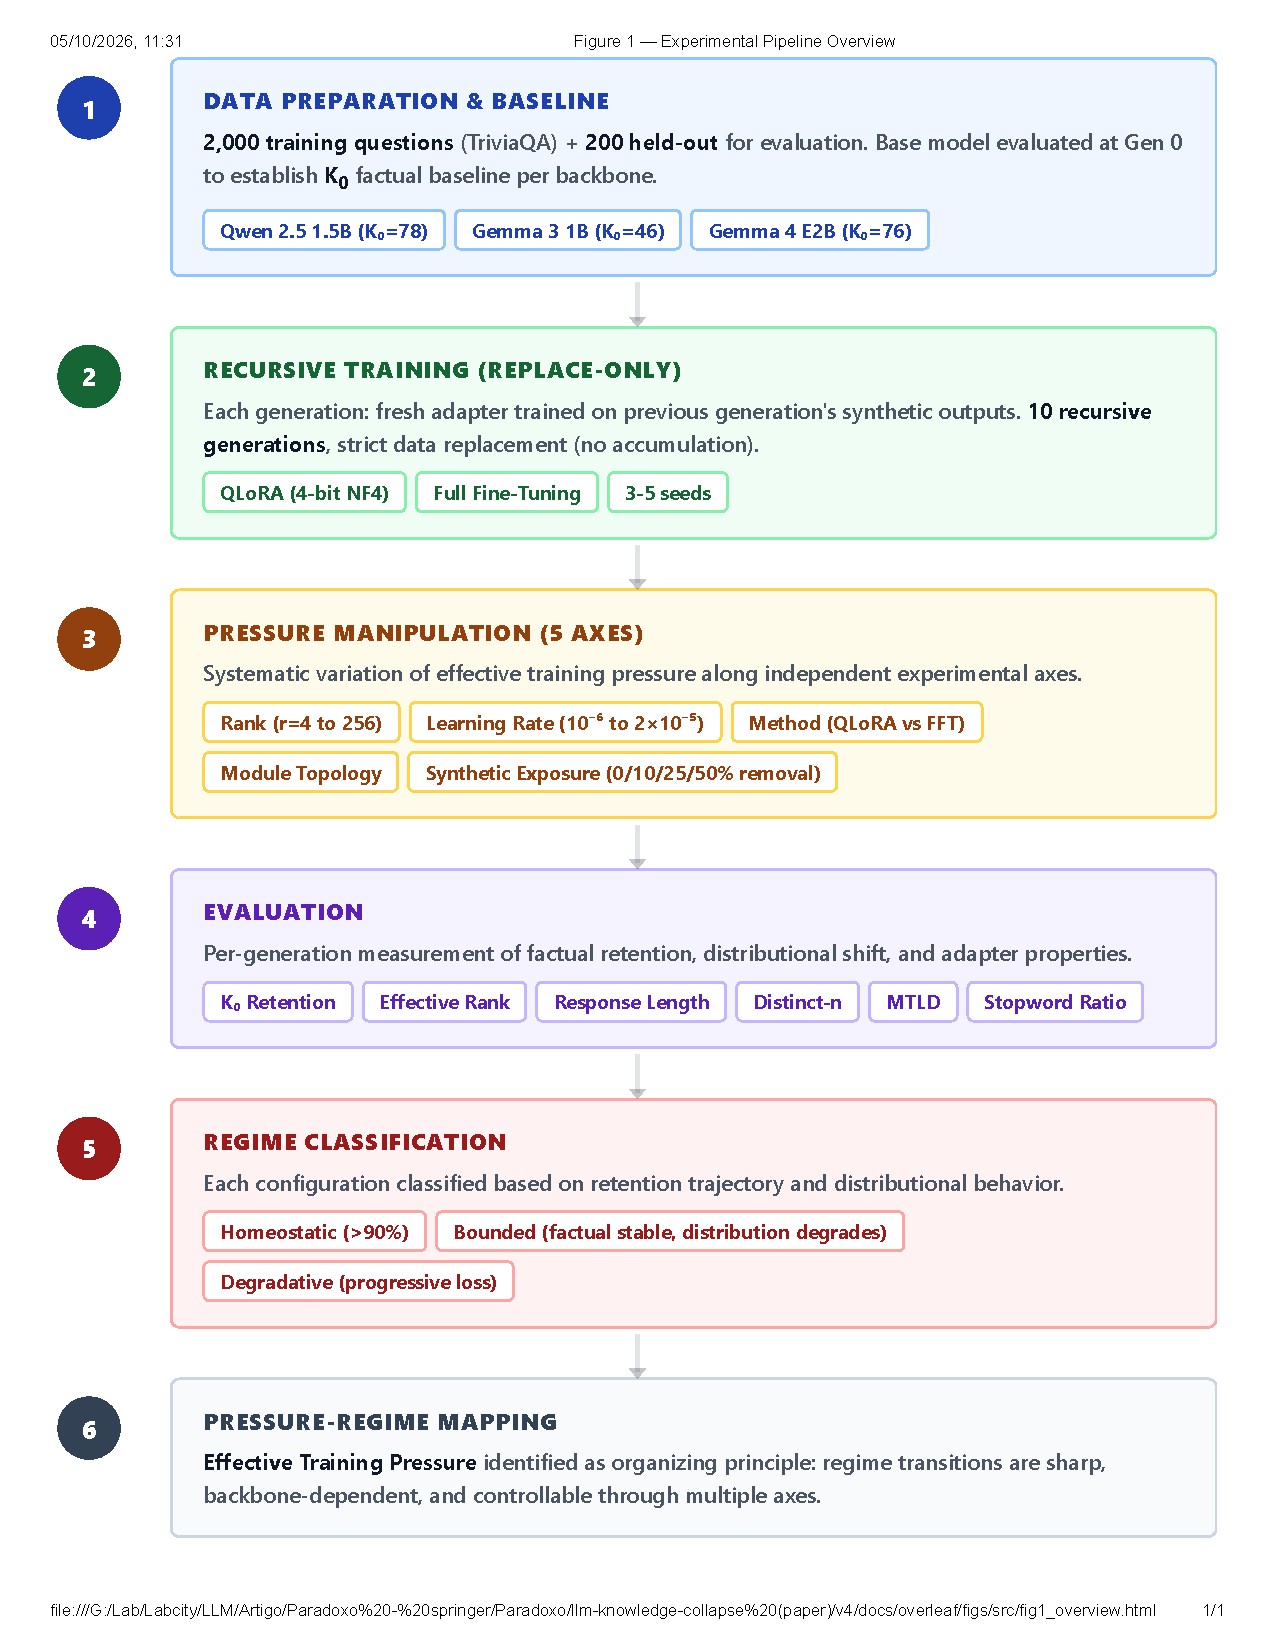
\includegraphics[width=0.98\textwidth]{figs/scratch/fig1_overview.pdf}%
  \vspace{4pt}
  \caption{Overview of the experimental pipeline: (1)~data preparation and
  $K_0$ baseline establishment; (2)~recursive training over ten generations
  across three backbones; (3)~pressure manipulation along five axes (rank,
  learning rate, method, module topology, exposure); (4)~evaluation of
  retention, distributional shift, and effective rank; (5)~regime
  classification; (6)~effective training pressure framework
  synthesis.}\label{fig:methodology}
\end{figure*}

\subsection{Experimental axes}\label{sec:axes}

Our dose-response design manipulates effective training pressure along five
experimental axes. Each axis targets a different component of pressure while
keeping the recursive protocol, dataset, and evaluation procedure fixed. The
axes are not intended to define a single scalar pressure value; rather, they
isolate how different sources of pressure, i.e., update capacity, perturbation
magnitude, module topology, and synthetic exposure, affect recursive stability.
Table~\ref{tab:axes} summarizes the experimental axes, the manipulated variable,
and the tested range.

\begin{table}[tp]
\caption{Experimental axes and their corresponding pressure
components.}\label{tab:axes}
\begin{tabular}{@{}cll>{\raggedright\arraybackslash}p{5.5cm}@{}}
\toprule
\# & Axis & Variable & Range \\
\midrule
1 & Capacity & QLoRA rank $r$ & $\{4, 16, 32, 64, 128, 256\}$ \\
2 & Magnitude & FFT learning rate & $10^{-6}$--$2{\times}10^{-5}$ \\
3 & Method & QLoRA vs FFT & Matched pert., $N{=}3$ \\
4 & Topology & Target modules & Attention vs full-linear \\
5 & Exposure & Training examples & \rev{0\%, 10\%, 25\%, 50\% removed (paired dose--response; B7/Qwen $r{=}256$, $n{=}5$; G2/Gemma~3 $r{=}10$, $n{=}3$)} \\
\bottomrule
\end{tabular}
\end{table}

The experimental design manipulates effective training pressure along five axes:

\begin{enumerate}
\item \textbf{Adapter rank (update capacity).} We vary QLoRA rank across six
values ($r=4,16,32,64,128,256$) on Qwen, producing adapters from 545K to 34.9M
trainable parameters. The headline ranks ($r=16$ and $r=256$) are evaluated with
three seeds; intermediate ranks trace the dose-response curve with a single
seed. On Gemma~3, we test $r \in \{4,10,12,14,16\}$ with five seeds at the
anchor ranks ($r=4$, homeostatic, and $r=16$, degradative) and a single seed at intermediate ranks.

\item \textbf{Learning rate (perturbation magnitude).} For full fine-tuning, we
sweep the learning rate across four logarithmically spaced values ($10^{-6}$,
$5{\times}10^{-6}$, $10^{-5}$, $2{\times}10^{-5}$), selected to span one
order of magnitude within the practical range commonly used for LLM
fine-tuning~\citep{hu2022,dettmers2023}. This range produced per-generation
weight drifts from 0.39 to 3.48 ($L_2$ norm), enabling perturbation-magnitude
dose-response analysis. This axis tests whether
perturbation magnitude drives the regime transition independently of adapter
rank.

\item \textbf{Method comparison (QLoRA vs FFT).} We compare QLoRA $r=16$
against FFT at $\mathrm{LR}=10^{-6}$, selected because it produces the closest
available perturbation proxy ($\|BA\|_F \approx 0.42$ vs FFT drift $\approx
0.39$). Because the LoRA Frobenius norm and the FFT weight drift measure
different geometric quantities, this constitutes a comparison at comparable
perturbation levels rather than an exact match. Both
are run for 10 generations with three seeds.

\item \textbf{Module topology (supportive ablation).} On Qwen, we compare
attention-only modules (\texttt{q\_proj}, \texttt{v\_proj}) with all linear
modules. This tests whether stability depends on module location or effective
update capacity. Single-seed; supportive evidence only.

\item \textbf{Synthetic exposure (intervention).} We manipulate the synthetic
training stream in the Qwen $r=256$ boundary regime. Interventions include
length filtering, and paired dose--response downsampling (0\%, 10\%, 25\%, 50\%
removal), and short-answer constraining. Design detailed in
Section~\ref{sec:intervention}.
\end{enumerate}

\subsection{Effective training pressure}\label{sec:pressure}

We use \textit{effective training pressure} as a conceptual framework for
interpreting recursive fine-tuning stability, rather than as a single fitted
equation. The term refers to the effective perturbation imposed on the model and
the synthetic training stream at each recursive generation. In our experiments,
this pressure arises from three jointly contributing factors:

\begin{enumerate}
    \item \textbf{Update capacity}: the dimensionality of the trainable update
    subspace, controlled by QLoRA rank and measured through effective rank.

    \item \textbf{Perturbation magnitude}: the size of the parameter update
    induced by one generation of training, controlled by learning rate in FFT and
    approximated by the norm of the composed LoRA update in QLoRA.

    \item \textbf{Synthetic exposure}: the amount and composition of
    model-generated training data fed back into the next generation, manipulated
    through filtering or downsampling of the synthetic stream.
\end{enumerate}

We do not assume a known functional form combining these components. Instead,
our experiments manipulate each component separately and show that changes along
any of the three axes can move the system between bounded and degradative
regimes.

\rev{We distinguish \emph{ETP-design} variables, which are fixed before training and
directly manipulated in our factorial design (nominal adapter rank $r$, learning
rate $\eta$, number of training steps, and synthetic-data dose fraction), from
\emph{ETP-observed} variables, which are measured after training as diagnostic
proxies (effective rank, mean absolute weight drift $d(t)$, response length, and
SDI-3). Effective rank and drift track how much pressure was actually applied to
the model, but they are not available prospectively; they therefore serve as
post-hoc explanatory variables rather than pre-specified predictors. The
operational index $\Pi = \mathrm{erank}(\Delta W) \times (\eta / 10^{-5})$ is reported as the mean across training generations, where $\mathrm{erank}(\Delta W)$ denotes the effective rank of the adapter weight update (see Table~\ref{tab:notation}). This is
an exploratory post-training summary and is not used as a validated quantitative
threshold.}

\subsubsection{Effective rank}\label{sec:erank}
To quantify update capacity beyond nominal rank, we compute the effective rank
of the composed LoRA update matrices $BA$ after training at each generation.
Following \citet{roy2007}, the effective rank is defined as
\begin{equation}\label{eq:erank}
    \mathrm{erank}(BA) =
    \exp\!\left(-\sum_i \hat{\sigma}_i \log \hat{\sigma}_i\right),
\end{equation}
where $\hat{\sigma}_i = \sigma_i / \sum_j \sigma_j$ are the normalized singular
values of $BA$. This measure captures how many singular directions carry
substantial weight in the adapter update. A rank-$r$ adapter with uniformly
distributed singular values reaches $\mathrm{erank}=r$, whereas an update
dominated by a single singular direction has $\mathrm{erank}\approx 1$ regardless
of nominal rank.

We report the mean effective rank across adapted
matrices in a model. For comparisons across module-targeting schemes, we also
consider aggregate effective rank, defined as the sum of effective ranks across
adapted matrices. In our within-backbone rank sweeps, effective rank generally
increases with nominal rank and organizes the observed transition between
stable and degradative regimes better than nominal rank alone. However,
raw effective-rank thresholds are not portable across architectures: Qwen
remains bounded at substantially higher effective ranks than Gemma~3. We
therefore treat effective rank as a within-backbone capacity measure and discuss
cross-architecture normalization as a limitation in Section~\ref{sec:limitations}.

\subsubsection{Perturbation magnitude}\label{sec:pertmag}
For full fine-tuning, we measure perturbation magnitude as the mean absolute
parameter change relative to the original model weights:
\begin{equation}\label{eq:drift}
    \rev{d(t)} =
    \frac{1}{|\theta|}\sum_i |\theta^{(t)}_i - \theta^{(0)}_i|.
\end{equation}
Here $\theta^{(0)}$ denotes the original model parameters and $\theta^{(t)}$
the parameters after one generation of fine-tuning.
% [v4] A6 RESOLVIDO: abs_drift = mean absolute por parâmetro, confirmado no código
This scalar summarizes the
average displacement of the model in weight space under FFT. For QLoRA, the
closest available perturbation proxy is the Frobenius norm of the composed
adapter update, $\|BA\|_F$. These two quantities are not geometrically identical:
one measures displacement of the full model weights, while the other measures
the magnitude of a low-rank update. We therefore use them only as approximate
perturbation proxies when selecting the FFT/QLoRA comparison in Axis~3.

\subsection{Output-distribution diagnostics}\label{sec:metrics}

Beyond factual retention, we track output-distribution diagnostics designed to
measure how the synthetic training stream changes across recursive generations.
These metrics serve two purposes. First, they detect distributional degradation
that may not be captured by K0 retention alone. Second, they provide monitorable
signals that could be used to audit recursive fine-tuning pipelines. We treat
these diagnostics as descriptive indicators of output drift, not as standalone
causal explanations for factual loss. We compute four complementary diagnostics.

\textit{Content efficiency} is defined as factual retention normalized by mean
response length:
\begin{equation}\label{eq:efficiency}
    \mathrm{ContentEff}(t) =
    \frac{\rev{R(t)}}{\mathrm{MeanLength}(t)}.
\end{equation}
Here, $\mathrm{MeanLength}(t)$ is measured in words over the generated synthetic
responses at generation~$t$. Declining content efficiency indicates that the
model produces more tokens per retained fact; stable content efficiency indicates
that retention and response length remain proportionally stable.

\textit{Baseline response persistence} compares the model's normalized response
at generation~$t$ with its response at generation~0:
\begin{equation}\label{eq:persistence}
    \mathrm{Persist}(t) =
    \frac{|\{q \in K_0 : a_t(q) = a_0(q)\}|}{|K_0|}.
\end{equation}
High persistence indicates responses remain anchored to generation-0 outputs.
Declining persistence indicates response drift even when aggregate retention
remains bounded.

\textit{Lexical diversity and verbosity} are measured using several corpus-level
metrics, motivated by prior characterizations of neural text degeneration
\citep{holtzman2020}. Distinct-$n$~\citep{li2016} computes the ratio of unique
$n$-grams to
total $n$-grams; we report Distinct-1 and Distinct-2. Because Distinct-$n$ is
sensitive to response length, we also compute
\rev{Measure of Textual Lexical Diversity (MTLD)}~\citep{mccarthy2010}, a length-robust diversity estimate. We additionally
track mean response length and stopword ratio to distinguish verbosity increase
from content-word diversity changes.

Finally, we define the \textit{Synthetic Drift Index} (SDI-3) to summarize
output-distribution change:
\begin{equation}\label{eq:sdi}
    \mathrm{SDI\text{-}3} =
    \log\frac{\mathrm{MeanLen}_T}{\mathrm{MeanLen}_0}
    + \log\frac{\mathrm{D1}_0}{\mathrm{D1}_T}
    + \Delta I\,,
\end{equation}
where $\mathrm{D1}_t$ denotes the \rev{Distinct-1 unigram diversity} of synthetic
responses at generation~$t$; $\mathrm{MeanLen}_t$ is the mean response length in
words at generation~$t$; $\Delta I = \mathrm{Instability}(T) -
\mathrm{Instability}(1)$; and $\mathrm{Instability}(t)$ denotes the fraction of
training items whose normalized response differs between generation~$t{-}1$ and
generation~$t$. The convention $0\log 0 = 0$ applies. The three terms correspond to verbosity increase, unigram
diversity decrease, and loss of item-level response stability. SDI-3 is not
proposed as a theoretical measure; it is an empirical summary statistic used to
compare output drift across experimental conditions.

These diagnostics complement K0 retention by measuring distributional properties
of the synthetic stream. K0 retention measures preservation of initially known
facts, whereas the output diagnostics measure whether the generated training
data remain short, lexically efficient, and anchored to the model's initial
responses. Throughout the paper, we interpret these metrics as signatures of
distributional drift. Causal claims are reserved for explicit interventions on
the synthetic training stream in Section~\ref{sec:intervention}.

\subsection{Synthetic-exposure interventions}\label{sec:intervention}

The interventions in Axis~5 test whether the degradative regime can be shifted
back toward homeostasis by reducing synthetic training exposure. The primary
evidence comes from two pre-registered dose--response experiments, one on each
backbone.

\textbf{Qwen dose--response (B7, $r=256$, $n=5$ seeds).}
Five paired seeds receive 0\%, 10\%, 25\%, or 50\% random downsampling of the
synthetic training stream. The 0\% arm serves as a within-pipeline baseline
(same evaluation code, same seeds), eliminating cross-pipeline confounds. The
pre-registration hash is \texttt{a916ebf}.

\textbf{Gemma~3 dose--response (G2, $r=10$, $n=3$ seeds).}
An independent pre-registered experiment applies the same four dose levels to
Gemma~3~1B~IT at $r=10$. The evaluation set is $|K_{0,\mathrm{G2}}|=44$ items
(established by the \texttt{g1\_rank10} pipeline; see Section~\ref{sec:k0}).

\rev{A prior exploratory pilot (C1--C5) used a qualitatively different
experimental design: five discrete intervention strategies (baseline, prompt
constraint, length filtering, canonical extraction, and random downsampling)
evaluated on a single seed with a different evaluation pipeline. When C1 and C5
from that pilot are re-run under an identical pipeline and paired seeds, the
approximate $5\%$ downsampling effect is $+1.9$\,pp ($n=3$), which is not
statistically distinguishable from zero. The pilot results are archived in the
replication repository; they are not used in the primary effect estimates below.}

\subsection{Seeds, statistics, and reporting}\label{sec:statistics}

Recursive fine-tuning experiments are computationally expensive because each
condition requires multiple generations of training and data regeneration. We
therefore use a small but explicit seed policy, distinguishing between
multi-seed headline comparisons and single-seed supporting ablations.

All headline comparisons are evaluated with multiple independent training seeds
(three for Qwen conditions, five for Gemma~3 anchor ranks). These
include the Qwen rank-sweep endpoints ($r=16$ and $r=256$), the Gemma~3 anchor
ranks ($r=4$, homeostatic, and $r=16$, degradative), the QLoRA--FFT comparison, and the dose--response synthetic
exposure interventions. Intermediate dose-response points and supporting
ablations are evaluated with a single seed and labeled as such. We do not pool
single-seed and multi-seed results when making headline claims.

For multi-seed conditions, we report per-seed values together with the mean and
observed range. When the observed ranges of two conditions do not overlap across
all seeds, we interpret this as evidence of consistent empirical separation
under the present experimental protocol.

We emphasize
effect sizes, ordinal dose-response behavior, and per-seed consistency. The
QLoRA rank sweep and FFT learning-rate sweep are interpreted as dose-response
curves across six and four levels respectively, where the ordinal consistency of
the entire sweep provides stronger evidence than any single pairwise comparison.

Effect sizes are reported as absolute percentage-point gaps in factual retention.
For QLoRA--FFT comparisons, gaps are reported per seed and as a mean. For
synthetic-exposure interventions, we report the improvement over the \rev{0\%-removed
within-pipeline baseline} at the same generation; the earlier C1--C5 pilot used a
different evaluation pipeline and is not used as the primary reference. We do not claim precise threshold locations
or a universal effective-rank value at which degradation begins; instead, we
identify the interval between adjacent tested settings where the regime
transition occurs. Single-seed observations are used as exploratory or
supportive evidence and are not used as standalone support for headline
conclusions.

\subsection{Sources of variation and experimental controls}\label{sec:controls}

Table~\ref{tab:controls} maps each potential source of variation in the
recursive fine-tuning setup to the experimental control used to address it.
This inventory responds directly to the question of whether observed regime
transitions might be attributable to confounds rather than to the manipulated
axis. Controls marked with a dedicated experiment (G3, G4) are evaluated
quantitatively in Section~\ref{sec:results}; the remaining entries rely on
held constant across all conditions within a backbone.


\begin{table}[H]
\caption{\rev{Sources of variation in the recursive fine-tuning protocol and
the corresponding experimental control. G3 and G4 refer to dedicated
within-session ablations (Section~\ref{sec:results}). ``Held constant''
denotes that the factor is fixed across all conditions for a given backbone.}}
\label{tab:controls}
\small
\begin{tabular*}{\columnwidth}{@{\extracolsep{\fill}}>{\raggedright\arraybackslash}p{3.5cm}>{\raggedright\arraybackslash}p{4cm}>{\raggedright\arraybackslash}p{3cm}@{}}
\toprule
\textbf{Source of variation} & \textbf{Potential confound} & \textbf{Control} \\
\midrule
Quantization (NF4 vs bf16) & Numerical noise from 4-bit quantization could inflate or suppress apparent degradation & G3: QLoRA bf16 (no NF4) vs QLoRA NF4, matched seeds \\
\addlinespace
Training data order & Shuffling artefacts could drive regime classification & G4: three independent shuffle seeds at fixed $r$=256 \\
\addlinespace
Optimizer state & Accumulated momentum could confound generation-to-generation comparisons & Held constant: fresh optimizer at every generation (no state carryover) \\
\addlinespace
Synthetic data seed & Stochastic generation could produce artefactual variation & Reported per seed; headline conditions use 3–5 independent seeds \\
\addlinespace
Backbone architecture & Regime thresholds may not generalise & Replicated on Gemma~3~1B~IT ($r \geq 10$ degradative) and Gemma~4~E2B~IT ($r$=64 degradative, $N$=1) \\
\addlinespace
Pipeline version & Different code paths could introduce discrepancies & Each experiment uses a dedicated script and commit; see the replication repository for the per-experiment manifest. \\
\addlinespace
Evaluation scoring leniency & Bidirectional substring criterion may inflate retention at high verbosity & Noted per condition; strict exact-match re-evaluation reported in supplementary Table~S2 \\
\bottomrule
\end{tabular*}
\end{table}

The results presented in Section~\ref{sec:results} follow the experimental
organization introduced above. They first examine capacity-gated regime
transitions (Axes~1--2), then compare QLoRA and full fine-tuning (Axis~3),
characterize the accompanying distributional signatures, and finally evaluate
exposure interventions (Axis~5). Module topology ablations (Axis~4) are
presented alongside the capacity analysis.

% ============================================================
% 4. RESULTS
% ============================================================
\section{Results}\label{sec:results}

The results are organized by experimental axis to examine how the main
components of effective training pressure relate to recursive stability and
degradation. We begin with the central empirical result: a clear, monotonic
regime transition as adapter rank increases on Qwen, which serves as the primary
backbone because it provides the highest-resolution dose-response
characterization through six rank levels evaluated across ten generations
(Section~\ref{sec:res_capacity}). We then evaluate whether the same behavior
generalizes across different model families (Section~\ref{sec:res_backbone}),
investigate whether increasing perturbation magnitude through full fine-tuning
reproduces the same dose-response pattern (Section~\ref{sec:res_fft}), characterize the
distributional signatures associated with above-threshold regimes
(Section~\ref{sec:res_distribution}), and present evidence that \rev{graded
reductions in synthetic exposure (50\% on both backbones) restore near-homeostatic
behavior at the regime boundary}
(Section~\ref{sec:res_intervention}). Throughout this section, headline findings are
supported by multi-seed experiments, whereas single-seed results are presented
as supporting evidence.

\begin{figure*}[t]
\centering
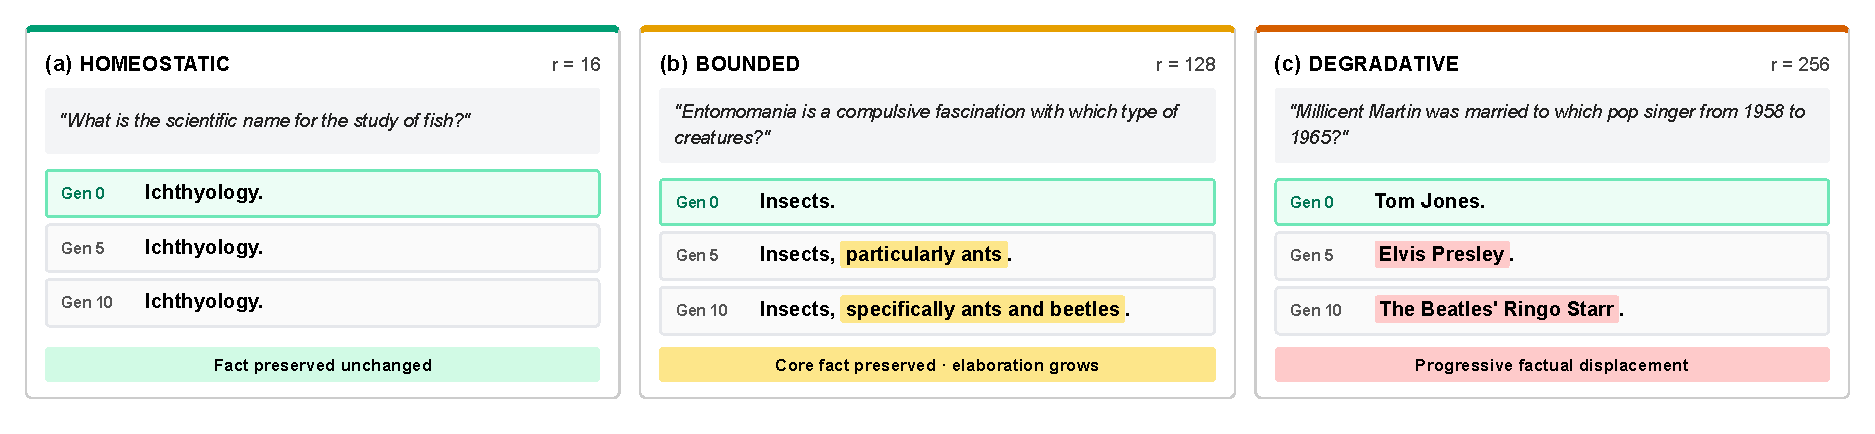
\includegraphics[width=0.95\textwidth]{figs/final/fig_regime_examples.pdf}
\caption{Representative response evolution under the three recursive regimes
(Qwen~2.5~1.5B, seed~15). Examples illustrate the characteristic behavior of
each regime: stable retention~(a), distributional drift with bounded
accuracy~(b), and progressive factual displacement~(c). Examples were selected
from the $K_0$ evaluation benchmark to illustrate the median behavior within
each regime classification.}\label{fig:regime_examples}
\end{figure*}

Figure~\ref{fig:regime_examples} illustrates how the same factual question
produces qualitatively different response trajectories across regimes: in~(a),
the correct answer persists unchanged; in~(b), the answer remains correct but
becomes embedded in increasingly verbose filler text; in~(c), the factual
content is progressively displaced by unrelated or fabricated information.

\subsection{Update capacity: rank dose-response}\label{sec:res_capacity}

Increasing adapter rank produces a clear, monotonic decline in factual retention
across the full rank sweep on Qwen~2.5~1.5B.
Table~\ref{tab:rank_sweep} summarizes K0 retention, effective rank, trainable
parameters, and regime classification for each tested configuration. Across the evaluated range, three descriptive contrasts are relevant and must be kept separate.
\rev{In the original single-seed rank sweep, the $r=16$ run retained 75 of 78
facts at Gen10 ($96.2\%$). The G1 replicate set at $r=256$ retained
$[61,\,63,\,61]$ of 78 facts across three seeds ($\GoneMten\% = 79.1\%$
mean). We therefore do not treat the single-seed $r=16$ value as a matched
replicate for $r=256$.}
\rev{For matched G3 bf16 pairs (same three seeds, same protocol, rank the only
variable), $r=16$ retained 76/78 in all three seeds while $r=256$ retained
$[61,\,63,\,61]/78$. The mean within-protocol gap is $18.4$\,pp; with $N{=}3$
pairs, the exact two-sided sign test gives $p{=}0.25$, so this result is
descriptive rather than confirmatory.}
\rev{For the six-seed G1$+$G4 estimate, $r=256$ retained
$\GoneFourMten\%\pm\GoneFourSDten$\,pp at Gen10, giving a cross-protocol
descriptive gap of $17.7$\,pp versus the three-seed G3 bf16 $r=16$ runs (each retaining 76/78); the two
protocols differ in quantization and seed assignment.}

\begin{table}[width=.95\linewidth,cols=7,pos=htbp]
\caption{QLoRA rank sweep on Qwen~2.5~1.5B-Instruct. The degradative endpoint
($r=256$) is replicated with three seeds to confirm
reproducibility.\textsuperscript{*} \rev{Retention for $r=4$ and $r=32$ is
reported at Gen5; all other configurations at Gen10.}}\label{tab:rank_sweep}
\begin{tabular*}{\tblwidth}{@{}l@{\hskip 4pt}l@{\hskip 4pt}l@{\hskip 4pt}l@{\hskip 4pt}l@{\hskip 4pt}l@{\hskip 4pt}l@{}}
\toprule
Rank ($r$) & Params & Gen & Retention & Eff.\ Rank & \rev{$N$} & Regime \\
\midrule
4   & 545K  & 5  & 97.4\%  & 3.34  & \rev{1} & \rev{Homeostatic} \\
16  & 2.2M  & 10 & 96.2\%  & 11.08 & \rev{1} & \rev{Homeostatic} \\
32  & 4.4M  & 5  & 96.2\%  & 17.85 & \rev{1} & \rev{Homeostatic} \\
64  & 8.7M  & 10 & 92.3\%  & 29.52 & \rev{1} & \rev{Homeostatic} \\
128 & 17.4M & 10 & 89.7\%  & 50.16 & \rev{1} & Bounded \\
256\textsuperscript{*} & 34.9M & 10 & 79.1\%  & 87.57 & \rev{3} & Degrad. \\
\bottomrule
\end{tabular*}
{\footnotesize \textsuperscript{*}Mean across three independent seeds.}
\end{table}

The longitudinal trajectories (Fig.~\ref{fig:trajectories}) reveal distinct
temporal dynamics across regimes.

\begin{figure}
  \centering
  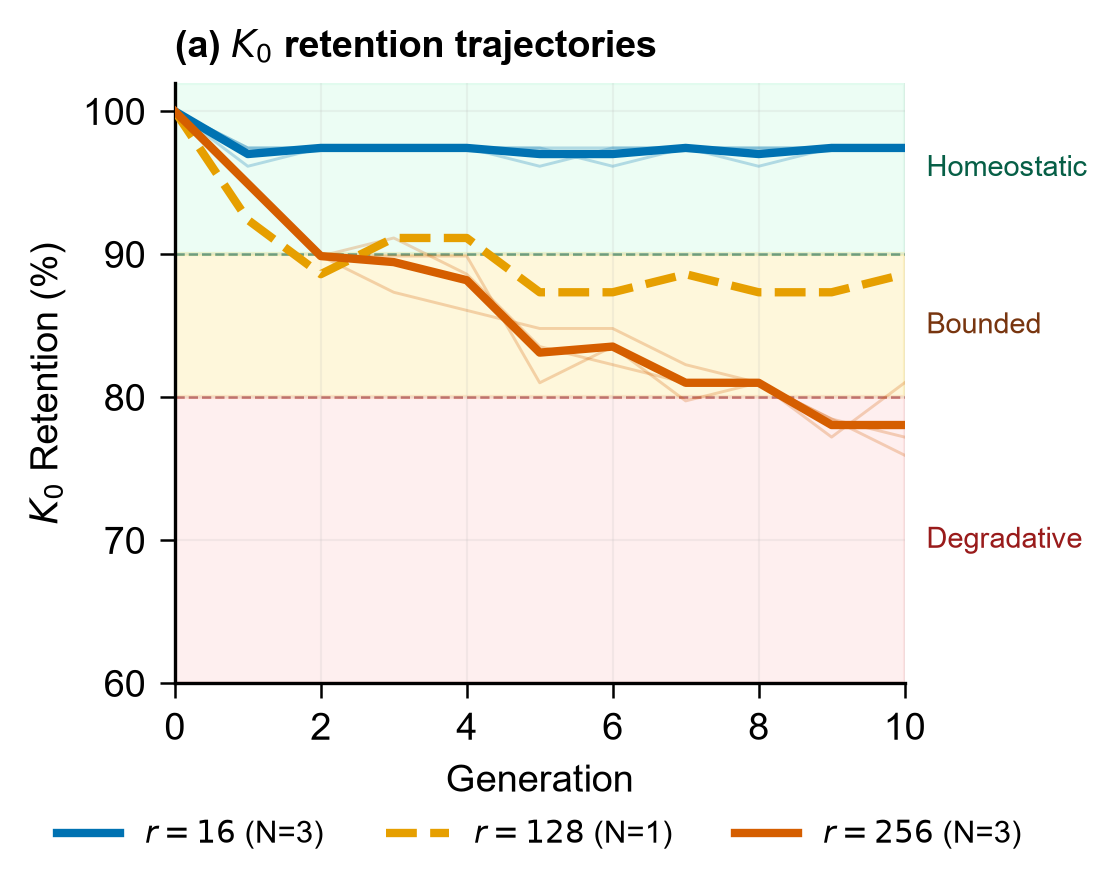
\includegraphics[width=0.95\columnwidth]{figs/final/fig1_trajectories.png}\\[4pt]
  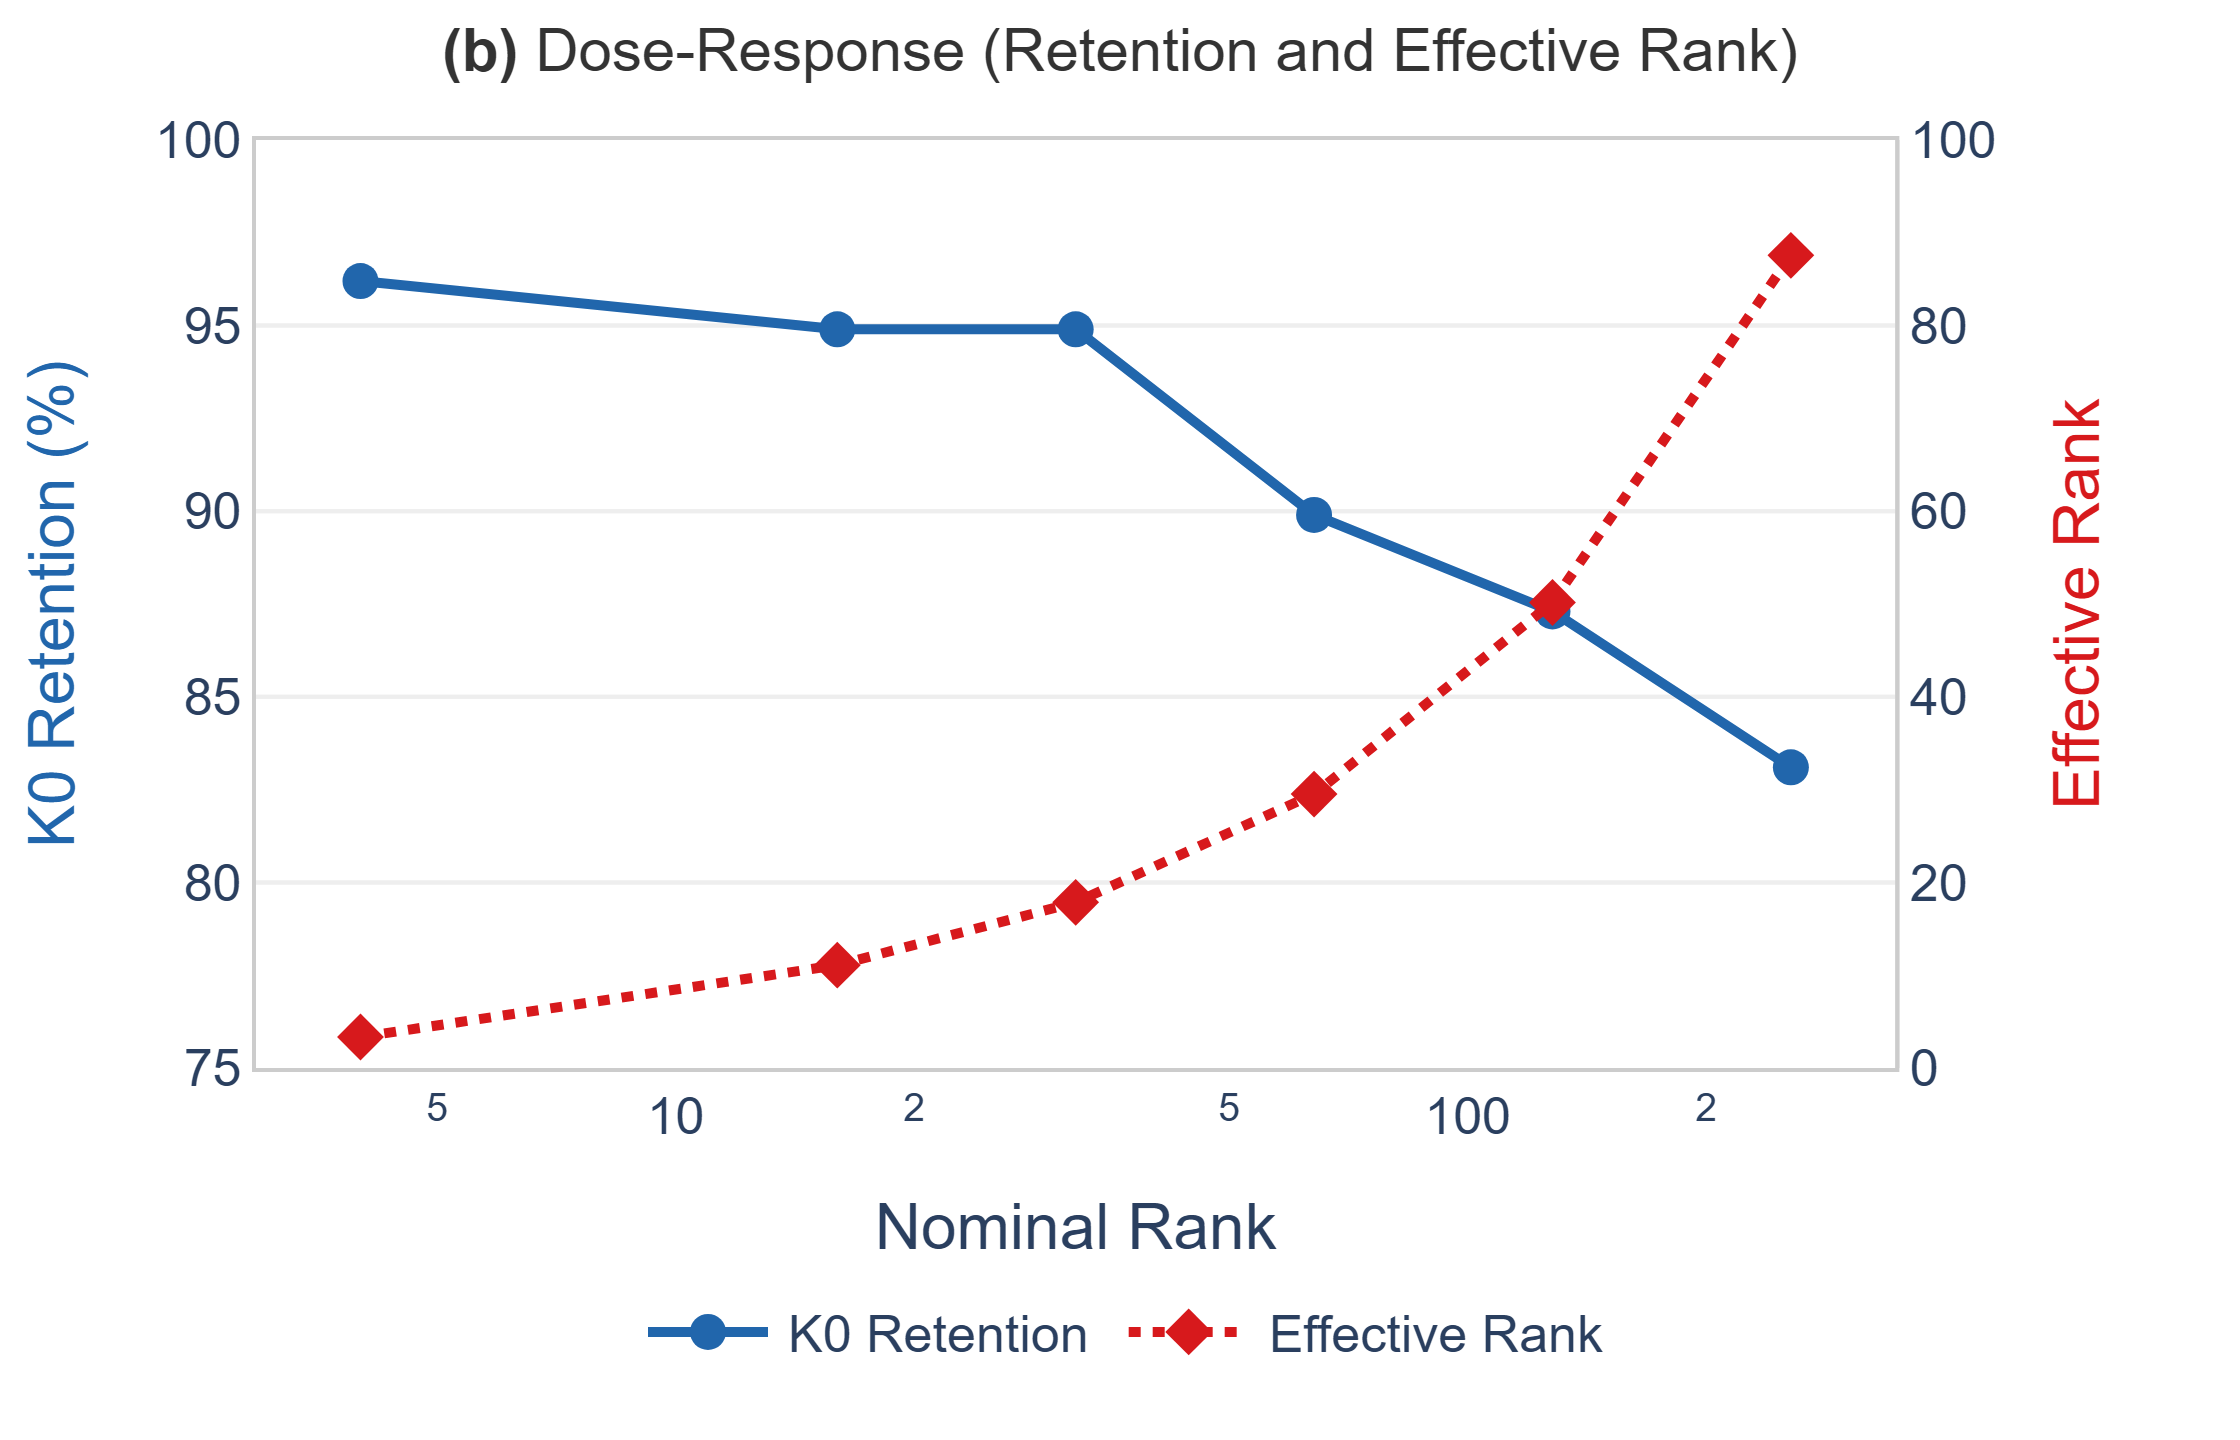
\includegraphics[width=0.95\columnwidth]{figs/final/fig2_dose_response.png}
  \caption{(a) K0 retention trajectories over 10 recursive
  generations for three representative ranks on Qwen~2.5~1.5B. Semi-transparent
  lines show individual seeds; solid thick lines show the per-rank mean.
  Background bands indicate regime classification (green: homeostatic,
  yellow: bounded, red: degradative). (b) Dose-response
  relationship: retention at last evaluated generation (Gen5 for $r=4$,$32$; Gen10 otherwise) versus nominal rank (left axis); mean effective
  rank versus nominal rank (right axis). Effective rank grows sub-linearly with
  nominal rank, indicating that increases in nominal capacity translate into
  progressively smaller increases in effective update
  dimensionality.}\label{fig:trajectories}
\end{figure}

At $r=16$, retention stabilizes after
an initial one-generation adaptation cost and remains flat through Gen10
(96.2\%). At $r=128$, retention settles at
88--89\% by Gen5 and remains bounded through Gen10, neither
recovering nor declining further. This bounded behavior distinguishes it from
both the stable regime and the progressively degradative regime. At
$r=256$, retention declines progressively,
% [v4] A7 — taxa corrigida: ~2 pp/gen era a média global incluindo Gen0→1.
% Inclinação pós-adaptação (Gen5→Gen10) é ~1.0 pp/gen para r=256.
reaching \rev{$\GoneFourMten\%$} (mean across \rev{six seeds, G1$+$G4}) by Gen10 with no sign of
stabilization within the observed horizon. The post-adaptation slope
\rev{(Gen5 to Gen10, $N=6$) is $\GoneSlope$~pp per generation.}

The dose-response curve (Fig.~\ref{fig:trajectories}b) reveals several
additional features. First, the
relationship between rank and retention is monotonically decreasing across all
six values, spanning more than an order of magnitude in trainable parameters
(545K to 34.9M). No rank reversal or non-monotonicity is observed. Second, the
decline accelerates at higher ranks: the gap between $r=64$ (92.3\%) and $r=256$
(79.1\%) is substantially larger than any gap between adjacent lower-rank
configurations. Third, effective rank increases sub-linearly with nominal rank
(3.34 at $r=4$ to 87.57 at $r=256$), indicating that higher-rank adapters do not
fully utilize their nominal capacity while still producing substantially larger
effective updates.

The multi-seed experiments at $r=256$ confirm that the degradative regime is
reproducible across independent training runs.
\rev{Combining the original three seeds (G1: seeds~15/137/256) with a three-seed
data-order control (G4: seeds~42/101/202), six independent $r=256$ runs
yield a Gen10 mean of $\GoneFourMten\%\pm\GoneFourSDten$~pp
(95\,\% CI $[\GoneFourCItenLo, \GoneFourCItenHi]$, range \GoneSeedFifteenTen--82.1\%).
The G1 three-seed mean alone is $\GoneMten\%\pm\GoneSDten$~pp
(95\,\% CI $[\GoneCItenLo, \GoneCItenHi]$).}
To verify that the homeostatic regime is also reproducible, we evaluated $r=16$
under the G3 bf16 protocol with the same three seeds (15/137/256); all three runs
returned \RsixteenMten\% Gen10 retention.
\rev{The cleanest seed-level rank comparison is the G3 within-protocol design,
where the same three seeds were run at both $r=16$ and $r=256$ under identical
bf16 precision. Per-seed Gen10 differences are $+15$, $+13$, and $+15$ correct
items out of 78, a mean of $+18.4$~pp. An exact sign-flip test gives $p=0.25$
($N=3$, bilateral); the effect is consistent in direction across all three pairs
but the sample size limits formal power.}
The arithmetic gap between the $r=16$ and $r=256$ conditions is
$\DeltaRanks$~pp ($r=16$: \RsixteenMten\%; $r=256$ G1$+$G4: $\GoneFourMten\%$),
demonstrating clear empirical separation under the present experimental protocol.

As a supportive ablation, we compared attention-only and full-linear module
targeting on Qwen at a single seed. Targeting all linear modules
(\texttt{q,k,v,o,gate,up,down}) at $r=4$ produces 4.6M trainable parameters and
96.2\% Gen5 retention, matching attention-only targeting at $r=16$ (2.2M
parameters, same retention). The full-linear $r=4$ adapter has a mean effective
rank of 3.43, compared to 11.08 for attention-only $r=16$. This preliminary
observation is consistent with effective update capacity, rather than module
location or parameter count alone, being the primary predictor of regime
membership. Because it is based on a single seed, we treat it as supportive
evidence.

Table~\ref{tab:transitions} summarizes item-level transitions across the rank
sweep. In the homeostatic regime, facts lost at one generation are recovered at
similar rates (net loss $\approx 0$), indicating bounded oscillation rather than
progressive forgetting. In the degradative regime, losses consistently exceed
recoveries, producing monotonic net displacement.

\begin{table}[tp]
\caption{Item-level transitions across recursive generations on
Qwen~2.5~1.5B (seed~15, $K_0 = 78$). C$\to$W (Correct$\to$Wrong): facts lost;
W$\to$C (Wrong$\to$Correct): facts recovered.}\label{tab:transitions}
\footnotesize
\renewcommand{\arraystretch}{1.4}
\begin{tabular}{@{}lcccc@{}}
\toprule
Rank & Gens & C$\to$W & W$\to$C & Net loss \\
\midrule
$r=4$   & 5  & 1  & 0 & 1 \\
$r=16$  & 10 & 3  & 3 & 0 \\
$r=32$  & 5  & 2  & 3 & $-$1 \\
$r=64$  & 10 & 7  & 7 & 0 \\
$r=128$ & 10 & 10 & 7 & 3 \\
$r=256$ & 10 & 19 & 4 & 15 \\
\bottomrule
\end{tabular}
\end{table}

The rank sweep and item-level transitions establish that increasing update
capacity through adapter rank is sufficient to produce a monotonic transition
from homeostatic to degradative recursive fine-tuning on the Qwen backbone. The
following sections examine whether this transition generalizes across
architectures and update mechanisms.

\subsection{Cross-backbone thresholds}\label{sec:res_backbone}

To test whether the regime transition observed on Qwen is architecture-specific,
we evaluated corresponding rank configurations on two additional backbones:
Gemma~3~1B, with five seeds at the boundary ranks over ten generations, and
Gemma~4~E2B, with a single seed across three ranks as additional validation.

\subsubsection{Gemma~3: cross-backbone replication}

On Gemma~3, an analogous regime structure emerges, but at a substantially lower
effective rank. Preliminary single-seed experiments identified the regime
boundary between $r=4$ (effective rank ${\sim}$3) and $r=16$ (effective rank
${\sim}$9); higher ranks were not evaluated with multiple seeds because $r=16$
already produces clear progressive degradation, making additional high-rank
conditions redundant for establishing the boundary location.
Table~\ref{tab:gemma3} summarizes the results. At $r=4$ (mean
effective rank 3.07), Gemma~3 remains stable across five seeds through ten
generations (mean Gen10 retention \rev{$\GthreeMtenRfour\%$, range 93.5--95.7\%}).
At $r=16$ (mean effective rank 9.2), Gemma~3 enters the degradative regime
across all five seeds (mean Gen10 retention \rev{$\GthreeMtenRsixteen\%$,
range 52.2--60.9\%}). The ranges do not
overlap at any generation from Gen1 onward, providing consistent empirical
separation between the two regimes on this backbone.

\rev{The mean difference is $\GthreeDeltaRanks$~pp (computed from raw item counts,
$K_0=\GthreeKzero$). Because the seed assignment across ranks is not confirmed
as paired in the archived data, we report two tests: if the same five seeds were
used at both ranks, the exact bilateral sign-flip test gives $p=0.0625$
($N=5$, all five differences positive); if seeds are independent, a bilateral
permutation test over $\binom{10}{5}=252$ allocations gives
$p=\GthreePermRanks$. The effect size is large (Hedges $g \approx \GthreeHedgesG$)
under either interpretation.}

Critically, the degradation at $r=16$ does not stabilize between Gen5 and
Gen10. Mean retention declines from 69.1\% at Gen5 to 56.5\% at Gen10, a
further loss of 12.6 percentage points with no sign of plateauing. This
progressive trajectory contrasts with the bounded behavior observed at $r=128$
on Qwen, where retention stabilizes near 89\%. The Gemma~3 $r=16$
configuration is therefore classified as progressively degradative rather than
bounded.

A notable feature of the degradative regime on Gemma~3 is that the mean
effective rank remains constant at approximately 9.2 throughout all ten
generations, even as retention declines from 85\% to 57\%. This suggests that
effective rank operates as a regime gate---determining whether the system
enters the degradative regime---rather than as a continuous predictor of the
rate of degradation within that regime.

To localize the threshold more precisely, we additionally evaluated intermediate
ranks $r \in \{10, 12, 14\}$ with a single seed. Intermediate ranks were
evaluated only to localize the transition boundary and were therefore not
extended to Gen10. All three exhibited progressive
degradation at Gen5: retention of 78.3\% ($r=10$, effective rank 6.37), 73.9\%
($r=12$, effective rank 7.35), and 69.6\% ($r=14$, effective rank 8.37). These
values place the Gemma~3 regime boundary between effective ranks 3 and 6.

\begin{table}[width=.95\linewidth,cols=6,pos=htbp]
\caption{QLoRA rank sweep on Gemma~3~1B~IT. Anchor ranks ($r=4$ and $r=16$),
representing the homeostatic and degradative regimes respectively,
are evaluated with five seeds over ten generations; intermediate ranks
($r=10,12,14$) with a single seed at Gen5 to localize the transition.}\label{tab:gemma3}
\begin{tabular*}{\tblwidth}{@{} llllll@{} }
\toprule
Rank & Gen & Retention & Eff.\ Rank & \rev{$N$} & Regime \\
\midrule
$r=4$   & 10 & 94.4\% (N=5) & 3.07  & \rev{5} & Homeostatic \\
$r=10$  & 5  & 78.3\%       & 6.37  & \rev{1} & Degradative \\
$r=12$  & 5  & 73.9\%       & 7.35  & \rev{1} & Degradative \\
$r=14$  & 5  & 69.6\%       & 8.37  & \rev{1} & Degradative \\
$r=16$  & 10 & 56.5\% (N=5) & 9.17  & \rev{5} & Degradative \\
\bottomrule
\end{tabular*}
\end{table}

\subsubsection{Gemma~4~E2B: additional validation}

To provide additional validation from a third model family, we evaluated
Gemma~4~E2B across three ranks ($r=4$, $r=16$, $r=64$) with a single seed
over ten generations. Table~\ref{tab:gemma4} summarizes the results.

The same monotonic dose-response structure emerges: $r=4$ (effective rank 2.04)
remains homeostatic at 94.7\% through Gen10; $r=16$ (effective rank 5.1)
exhibits bounded behavior at 88.2\%; and $r=64$ (effective rank 13.3)
enters the degradative regime, declining to 75.0\% by Gen10. The $r=64$
configuration additionally exhibits the same distributional drift pattern
observed in the Qwen degradative regime: mean response length inflates from
3.6 to 4.4 words, Distinct-1 collapses from 0.55 to 0.43, and stopword ratio
increases from 0.23 to 0.28.

Because these results are based on a single seed, we treat them as additional
qualitative validation rather than as a precise threshold estimate. The key
observation is that a third backbone, from a different model family, exhibits
the same regime structure under increasing adapter rank.

\begin{table}[width=.95\linewidth,cols=5,pos=htbp]
\caption{QLoRA rank sweep on Gemma~4~E2B~IT (seed~15, Gen10). Single-seed
results provide additional validation of the dose-response
structure.}\label{tab:gemma4}
\begin{tabular*}{\tblwidth}{@{} lllll@{} }
\toprule
Rank & Retention & Eff.\ Rank & $|K_0|$ & Regime \\
\midrule
$r=4$   & 94.7\% & 2.04  & 76 & Homeostatic \\
$r=16$  & 88.2\% & 5.10  & 76 & Bounded \\
$r=64$  & 75.0\% & 13.28 & 76 & Degradative \\
\bottomrule
\end{tabular*}
\rev{{\footnotesize All runs single seed (seed 15).}}
\end{table}

\subsubsection{Cross-backbone comparison}

Figure~\ref{fig:combined_traj} presents the retention trajectories for all three
backbones, enabling direct visual comparison of the regime structure across
architectures.

\begin{figure*}[t]
  \centering
  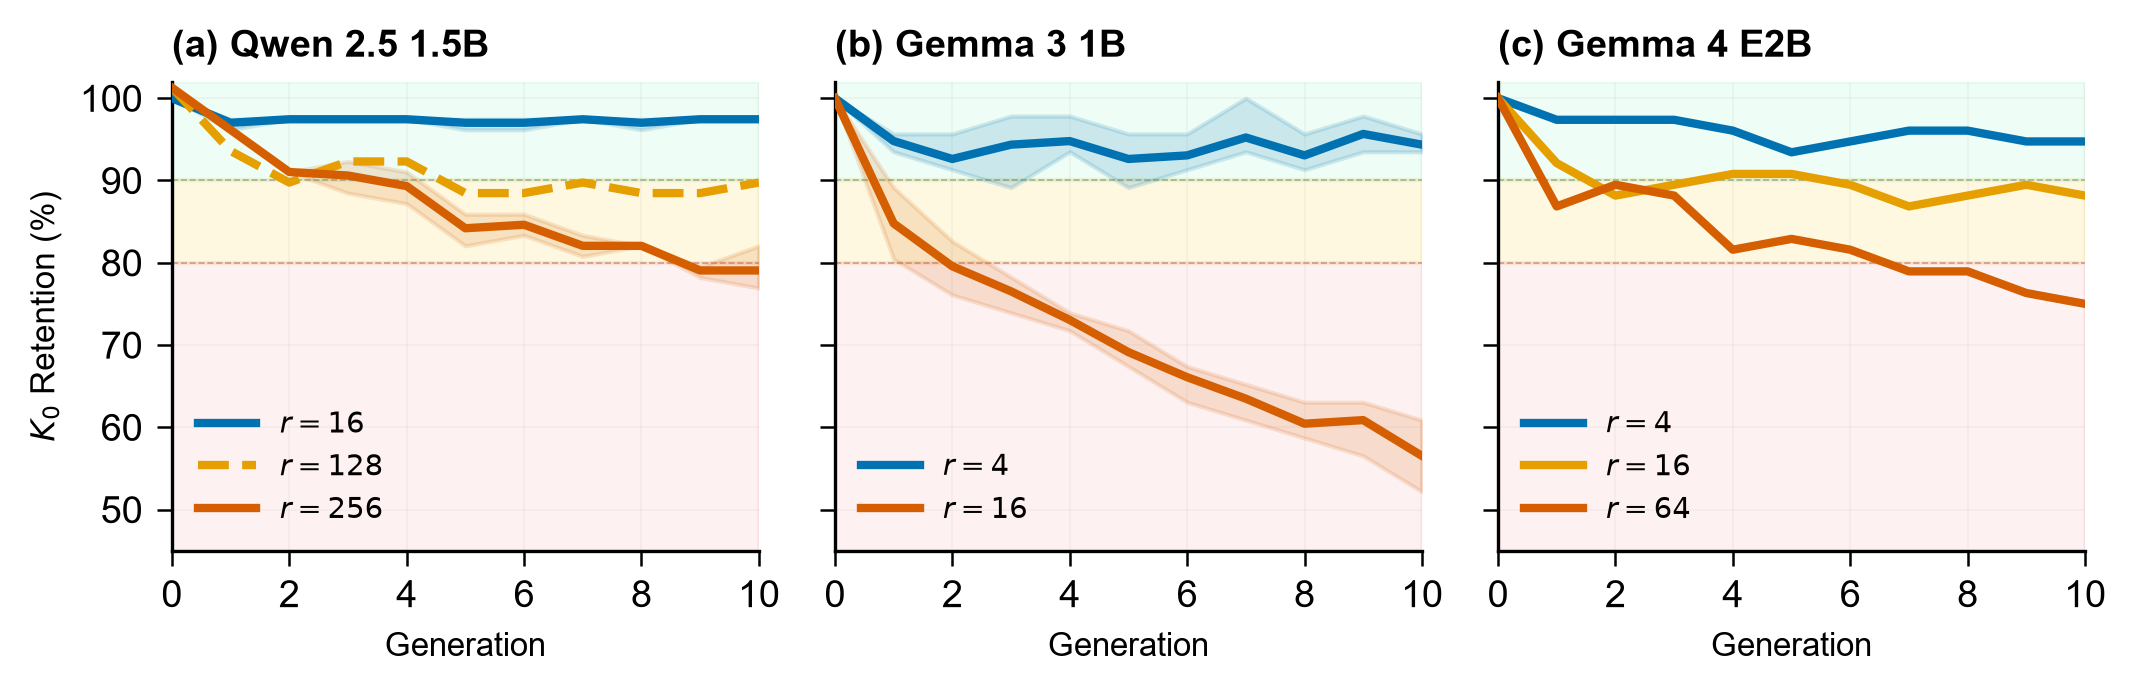
\includegraphics[width=0.95\textwidth]{figs/scratch/fig_combined_trajectories.png}
  \caption{$K_0$ retention trajectories over ten recursive generations across
  three backbones: (a)~Qwen~2.5~1.5B, (b)~Gemma~3~1B, and (c)~Gemma~4~E2B.
  Shaded bands show the range across seeds (N=5 for Gemma~3, N=3 for Qwen, N=1 for Gemma~4);
  solid lines show means. All three backbones exhibit consistent
  regime structure (homeostatic below threshold, degradative above), with the
  transition occurring at backbone-dependent effective-rank
  values.}\label{fig:combined_traj}
\end{figure*}

The homeostatic-to-degradative regime transition is observed consistently across
all three evaluated backbones, with consistent structure: bounded or
stable retention below the threshold, progressive degradation above. However,
the threshold location differs substantially across architectures. The Gemma~3
boundary lies between effective ranks 3 and 6, roughly an order of magnitude
below the Qwen threshold (between effective ranks 50 and 88). The E2B threshold
falls between effective ranks 5 and 13, intermediate between the other two
backbones. This ordering does not correspond simply to model size
(Gemma~3~1B < Qwen~1.5B < E2B~2B), indicating that the threshold is influenced
by architectural or pretraining properties not captured by parameter count
alone.

An attempt was made to normalize effective-rank thresholds across architectures by
dividing by hidden dimension, number of layers, number of attention heads, and
baseline diversity. None of these normalizations reduced the discrepancy to a
common threshold. We report this as a negative result and discuss it further in
Section~\ref{sec:limitations}.

\begin{figure}
  \centering
  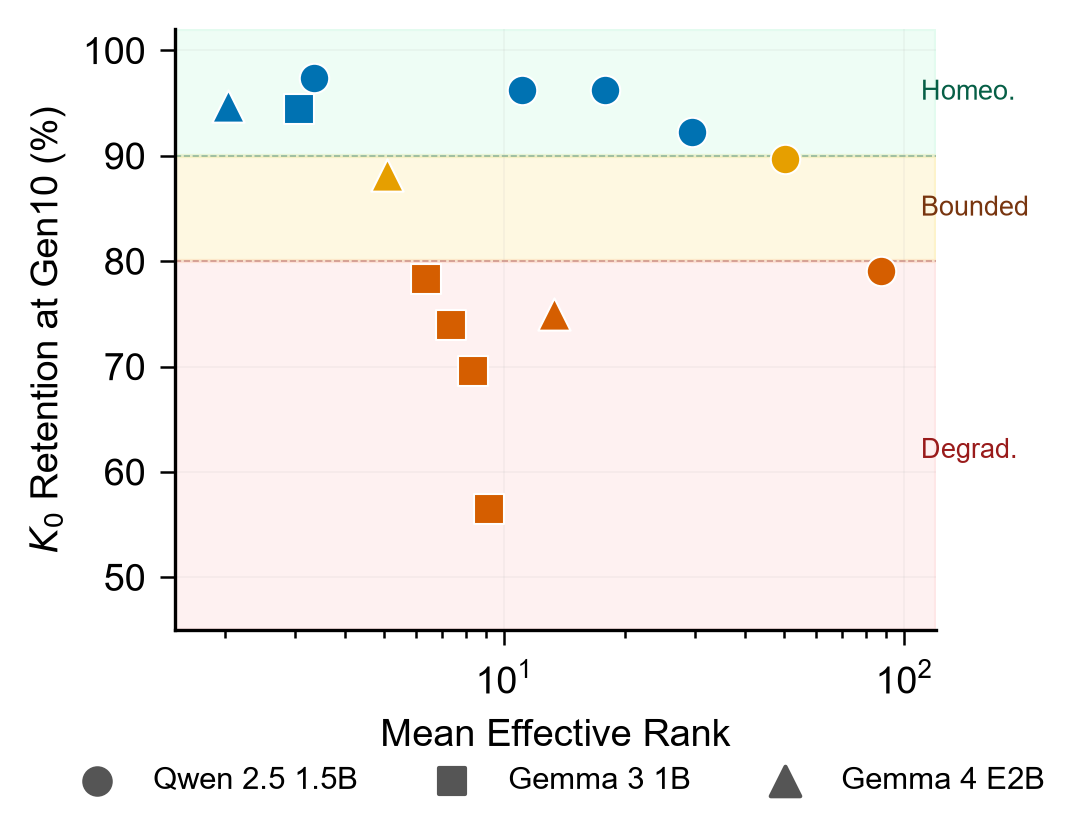
\includegraphics[width=0.95\columnwidth]{figs/scratch/fig_cross_backbone.png}
  \caption{$K_0$ retention versus mean effective rank across three backbones.
  Marker shapes distinguish backbones (circle: Qwen, square: Gemma~3, triangle:
  E2B); colors indicate regime membership (blue: homeostatic, orange:
  bounded, red: degradative). The regime transition occurs at
  substantially different effective-rank values across
  architectures.}\label{fig:cross_backbone}
\end{figure}

Having established that the regime structure generalizes across architectures,
with the key visual features visible in Figure~\ref{fig:cross_backbone}: (i)~all
three backbones exhibit a transition from blue (homeostatic) to red
(degradative) markers as effective rank increases; (ii)~the transition occurs at
substantially different x-axis positions across backbones; and (iii)~the Qwen
curve remains in the homeostatic region at effective ranks where Gemma~3 is
already fully degradative. We next examine whether the same transition occurs
when perturbation magnitude is varied independently of adapter capacity.

\subsection{Perturbation magnitude: FFT comparison}\label{sec:res_fft}

The previous sections established that increasing update capacity through adapter
rank shifts the system from homeostatic to degradative regimes. This section asks
whether increasing perturbation magnitude through full fine-tuning, without
varying adapter rank, reproduces an analogous dose-response pattern.

The learning rate was swept across four values on Qwen~2.5~1.5B under the same
recursive replace-only protocol. Table~\ref{tab:fft_sweep} shows retention
at Gen3, the earliest generation at which consistent regime separation emerges across
all four learning rates. Retention decreases monotonically as learning rate and weight drift increase. Drift
values span nearly an order of magnitude (0.39 to 3.48), and retention decreases
from 92.3\% to 84.6\% across this range. These results indicate that
perturbation magnitude alone can drive the system toward degradation without any
adapter or rank constraint.

\begin{table}[width=.95\linewidth,cols=4,pos=htbp]
\caption{FFT learning-rate sweep on Qwen~2.5~1.5B (seed~15, Gen3). Perturbation
proxy is the mean absolute weight drift relative to the original model for FFT,
and $\|BA\|_F$ for QLoRA. These are operationally comparable but not
geometrically identical measures. QLoRA~$r=16$ is included as a reference
point.}\label{tab:fft_sweep}
\begin{tabular*}{\tblwidth}{@{} llll@{} }
\toprule
Method & LR & Pert.\ proxy & Gen3 Retention \\
\midrule
QLoRA $r=16$ & $10^{-5}$          & 0.42\,($\|BA\|_F$) & 96.2\% \\
FFT          & $10^{-6}$          & 0.39               & 92.3\% \\
FFT          & $5{\times}10^{-6}$ & 1.56               & 91.0\% \\
FFT          & $10^{-5}$          & 1.95               & 89.7\% \\
FFT          & $2{\times}10^{-5}$ & 3.48               & 84.6\% \\
\bottomrule
\end{tabular*}
\rev{{\footnotesize QLoRA $r=16$ and FFT LR\,$=10^{-6}$: $N=3$ seeds. All other rows: $N=1$ seed (seed~15).}}
\end{table}

\subsubsection{QLoRA versus FFT at matched perturbation}
To compare the two update mechanisms at similar perturbation, we selected FFT at
LR$\,=10^{-6}$ (drift 0.39) as the closest available match to QLoRA $r=16$
($\|BA\|_F \approx 0.42$). Both were run for 10 generations with three seeds.
As illustrated in Figure~\ref{fig:fft_qlora}, the separation between the
trajectories is established after the first recursive generation and remains
nearly constant thereafter.

\begin{figure}
  \centering
  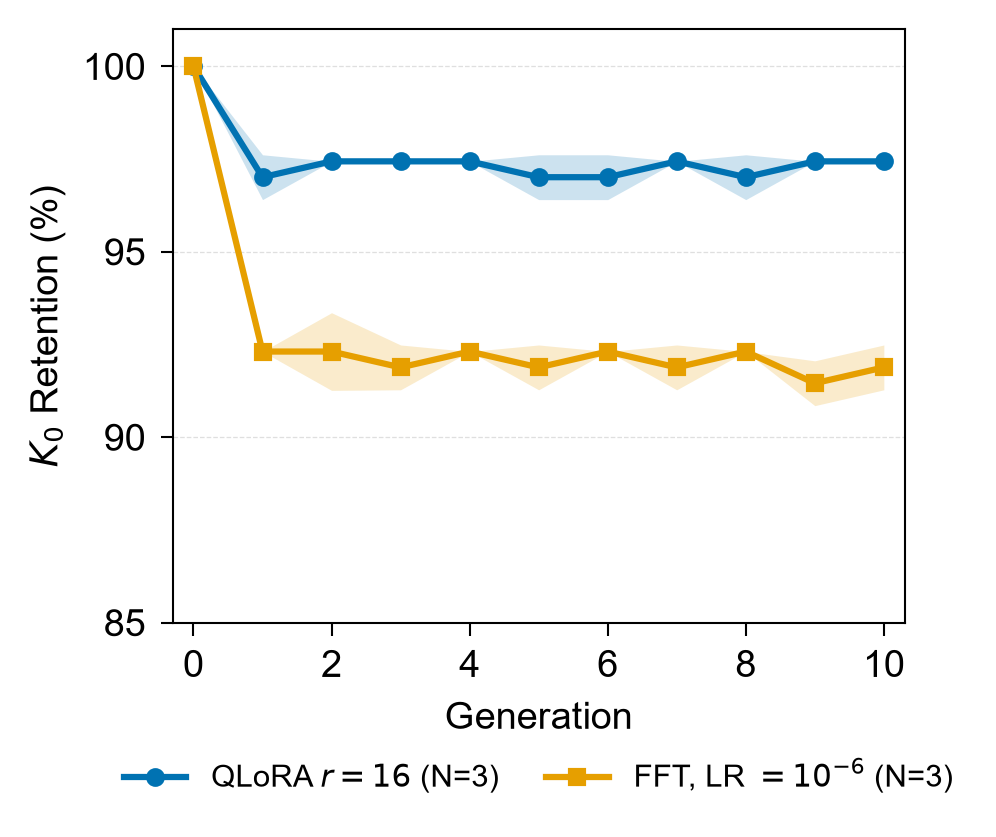
\includegraphics[width=0.95\columnwidth]{figs/final/fig4_fft_vs_qlora.png}
  \caption{$K_0$ retention over 10 recursive generations for QLoRA $r=16$ and
  FFT at LR$\,=10^{-6}$ on Qwen~2.5~1.5B. Lines show the mean across three
  seeds; shaded bands indicate $\pm$1 standard deviation.}\label{fig:fft_qlora}
\end{figure}

Both methods are stable from Gen1 through Gen10, with no progressive degradation
within the observed horizon. QLoRA retains a consistent advantage of
approximately 5.6 percentage points (mean Gen10: QLoRA 97.4\% vs FFT 91.9\%).
This gap emerges entirely at Gen1 and does not widen over subsequent generations.
This result is therefore interpreted as a difference in one-time adaptation cost rather than
a differential degradation rate: FFT incurs a larger initial factual cost when
adapting to the synthetic stream, while both methods exhibit similarly stable
trajectories once adapted.

QLoRA Gen10 retention is 97.4\% across all three seeds; FFT achieves
91.9\% (range 91.0--92.3\%). The ranges do not overlap across any seed pairing.

Item-level analysis reveals an asymmetry between the two methods. Under FFT, the
same six $K_0$ items are lost across all three seeds (cross-seed Jaccard
similarity 1.0), indicating a deterministic fragile-fact floor: these facts are
consistently displaced by full-parameter updates regardless of seed. Under
QLoRA, only two to three facts are lost per seed, and the overlap between facts
lost by QLoRA and facts lost by FFT is zero across all seed pairs (Jaccard 0.0).
In this low-perturbation regime, low-rank adaptation loses fewer facts and loses
different facts than full fine-tuning at comparable perturbation magnitude.

This pattern is referred to as a stable fragile-fact floor under FFT: certain facts
are reliably displaced by full-parameter updates, whereas low-rank updates
preserve those same facts while occasionally losing others. This observation is
consistent with prior work suggesting that LoRA and full fine-tuning can produce
qualitatively different update patterns even when achieving similar downstream
performance \citep{shuttleworth2024illusion,biderman2024}. The precise
mechanistic basis of this divergence in the recursive setting remains an open
question for future work.

\subsubsection{\rev{Rank and learning rate: joint dependence}}

The preceding analyses vary adapter rank and learning rate independently. To
test whether their effects are additive or interactive, we evaluated a
$3 \times 3$ matrix on Qwen: ranks 16, 64, and 256 crossed with learning rates
$5 \times 10^{-6}$, $10^{-5}$, and $2 \times 10^{-5}$. Table~\ref{tab:ranklr}
reports Gen5 retention for each cell, chosen as the common evaluation horizon
adopted for the Gemma~3 experiments, enabling cross-backbone comparison.

\begin{table}[width=.95\linewidth,cols=4,pos=htbp]
\caption{Rank $\times$ learning rate joint-dependence matrix on Qwen~2.5~1.5B
(retention evaluated at Gen5; $K_0 = 78$ items defined at generation~0, seed 15).}\label{tab:ranklr}
\begin{tabular*}{\tblwidth}{@{} llll@{} }
\toprule
Rank & LR=$5{\times}10^{-6}$ & LR=$10^{-5}$ & LR=$2{\times}10^{-5}$ \\
\midrule
$r=16$  & 76/78 (97.4\%) & 76/78 (97.4\%) & 72/78 (92.3\%) \\
$r=64$  & 76/78 (97.4\%) & 72/78 (92.3\%) & 69/78 (88.5\%) \\
$r=256$ & 70/78 (89.7\%) & 66/78 (84.6\%) & 64/78 (82.1\%) \\
\bottomrule
\end{tabular*}
\rev{{\footnotesize All cells: $N=1$ seed (seed~15).}}
\end{table}

\rev{The joint dependence} is evident (Figure~\ref{fig:heatmap}): configurations that remain stable under one
learning rate become bounded or degradative under another. At $r=16$, only
$\mathrm{LR}=2 \times 10^{-5}$ pushes the system below 95\% retention. At
$r=64$, the same degradation appears already at $\mathrm{LR}=10^{-5}$. At
$r=256$, even the lowest evaluated learning rate ($5 \times 10^{-6}$) produces
measurable degradation (89.7\%). Conversely, reducing learning rate partially
offsets the effect of higher rank: $r=256$ with $\mathrm{LR}=5 \times 10^{-6}$
retains 89.7\%, compared to 84.6\% at $\mathrm{LR}=10^{-5}$ and 82.1\% at
$\mathrm{LR}=2 \times 10^{-5}$. This demonstrates that the observed regime
depends jointly on update capacity and perturbation magnitude rather than on
either axis in isolation.

\begin{figure}
  \centering
  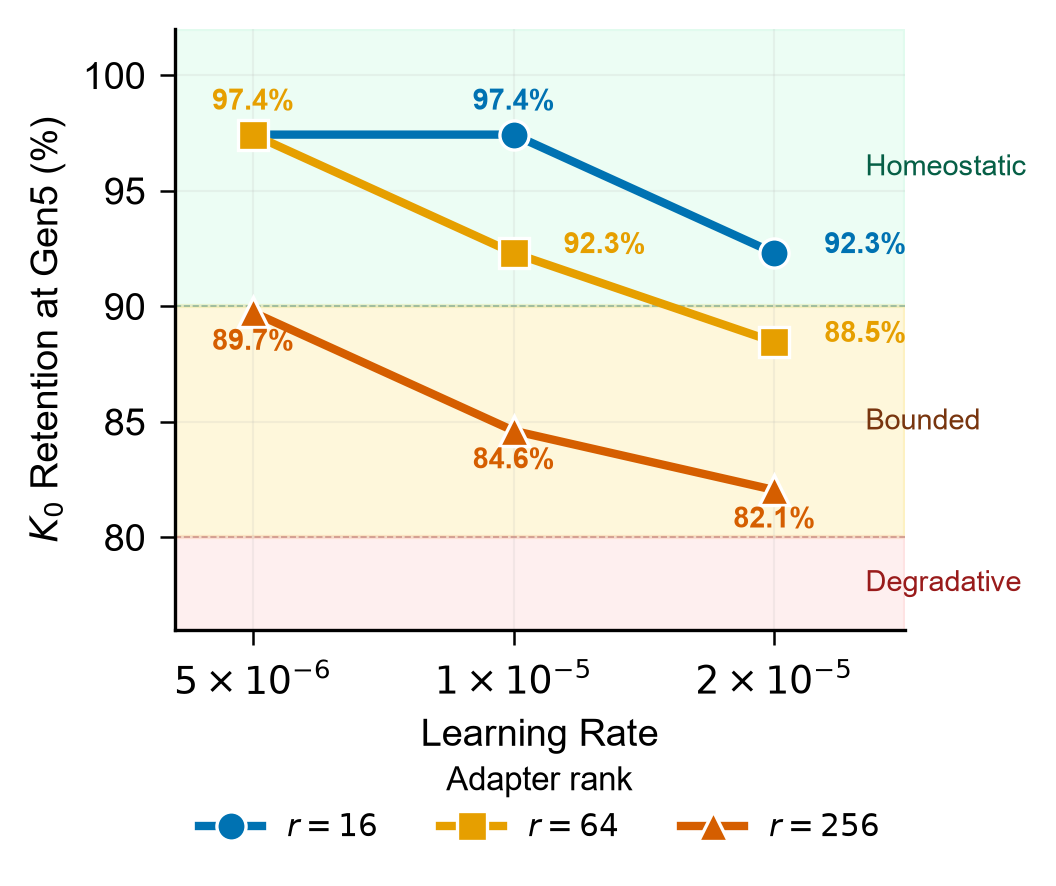
\includegraphics[width=0.95\columnwidth]{figs/final/fig_rank_lr_heatmap.png}
  \caption{Rank $\times$ learning-rate joint pattern on Qwen~2.5~1.5B
  (Gen5 retention). Non-parallel slopes indicate that rank and learning rate
  jointly determine the operating regime: higher rank amplifies the effect of
  increased learning rate, and vice versa.}\label{fig:heatmap}
\end{figure}

\subsubsection{
\rev{FFT on Gemma~3 is consistent with a cross-backbone magnitude effect}}

To test whether the perturbation-magnitude axis generalizes beyond Qwen, we
evaluated full fine-tuning on Gemma~3~1B at three learning rates. Gen5 retention
was 78.3\% at $\mathrm{LR}=10^{-6}$, 54.3\% at $\mathrm{LR}=5 \times 10^{-6}$,
and 63.0\% at $\mathrm{LR}=10^{-5}$. Although the two higher learning rates do
not follow a strictly monotonic pattern (possibly reflecting single-seed
variability), substantially higher degradation is observed at larger learning
rates compared to $\mathrm{LR}=10^{-6}$. \rev{This exploratory single-seed result is consistent with the perturbation-magnitude
axis operating on Gemma~3 as well, but the non-monotonic pattern at $\mathrm{LR}=5\times10^{-6}$
limits interpretation. We treat this as descriptive evidence rather than
confirmatory generalization.}

Both update capacity (Axis~1) and perturbation magnitude (Axis~2) each produce
dose-response relationships with factual retention, and these axes interact
rather than operating independently. The regime transition therefore reflects a
multidimensional pressure landscape in which multiple control variables jointly
determine recursive stability. The next section examines how these regimes
manifest in the distributional properties of the synthetic outputs.

\subsection{Distributional signatures of degradation}\label{sec:res_distribution}

The previous sections identified regime transitions through factual retention
alone. This section asks how these regimes manifest in the distributional
properties of the synthetic outputs. We apply the output-distribution diagnostics
defined in Section~\ref{sec:metrics} to three representative Qwen configurations
selected from the rank sweep: $r=16$, which exhibited homeostatic behavior;
$r=128$, which exhibited bounded retention; and $r=256$, which exhibited
progressive degradation.

\subsubsection{Homeostatic regime ($r=16$)}
In the homeostatic regime, all distributional metrics remain stable across ten
generations. Mean response length increases only slightly (2.47 to 2.70 words),
Distinct-1 remains above 0.63, MTLD stays above 2000, stopword ratio remains
near 0.16, and baseline response persistence holds steady at approximately 36\%.
Content efficiency declines modestly from 0.41 to 0.35, reflecting the initial
one-generation adaptation cost but no progressive drift.

\subsubsection{Bounded regime ($r=128$)}\label{sec:dissociation}
The $r=128$ configuration reveals a dissociation between factual retention and
output-distribution quality. While K0 retention remains bounded at 89.7\% through
Gen10, the output distribution degrades substantially: mean response length
inflates from 2.47 to 7.0 words, content efficiency collapses from 0.41 to 0.13
(a threefold dilution), stopwords double from 12\% to 25\%, MTLD collapses from
2673 to 745, and baseline persistence falls to 5.2\%. We refer to this as a
\textit{filler verbosity} phenotype: the model pads responses with repetitive
function words while retaining enough factual content to maintain bounded
retention.

This dissociation has a practical implication: K0 retention alone does not fully
capture the onset of distributional degradation. A system monitored solely by
factual accuracy would classify $r=128$ as stable, while its generated outputs
have already degraded substantially in efficiency, diversity, and response
anchoring.

\subsubsection{Degradative regime ($r=256$)}
At $r=256$, nearly all metrics diverge from their baseline values. Mean response
length increases from 2.47 to 3.6 words, content efficiency declines from 0.41
to 0.22, and baseline response persistence collapses from 33\% to 3.8\% by
Gen10. Notably, MTLD \textit{increases} (2673 to 3804) and stopword ratio
\textit{decreases} (12\% to 9\%), indicating that the model generates more
varied vocabulary while losing factual anchoring. We refer to this as an
\textit{elaborative drift} phenotype: the model produces longer, lexically
diverse, but factually unanchored responses.

The two above-threshold configurations therefore exhibit distinct distributional
failure modes despite both departing from stable behavior: $r=128$ degrades
through filler accumulation, while $r=256$ degrades through elaborative
dispersion.

These observations motivate a descriptive three-regime taxonomy:

\begin{enumerate}
    \item \textbf{Homeostatic} ($r \leq 64$ on Qwen, retention above
    approximately 90\%): factual retention and output-distribution metrics are
    both stable.
    \item \textbf{Distributionally degraded, factually bounded} ($r=128$ on
    Qwen): factual retention remains bounded while output-distribution metrics
    degrade substantially.
    \item \textbf{Factually degradative} ($r=256$ on Qwen): factual retention
    declines progressively and output distribution drifts.
\end{enumerate}

This taxonomy summarizes the observed behavior of the evaluated configurations
rather than defining universally distinct categories. The empirically observed rank intervals separating regimes are $r_H \in (64, 128)$ and $r_D \in (128, 256)$ (Qwen-specific observations, not universal thresholds).
The degradative regime
($r=256$) is qualitatively consistent with the Stage~B ``knowledge collapse''
described by \citet{keisha2025}, where fluency persists while factual accuracy
deteriorates. The distributionally degraded regime ($r=128$), however, represents
a condition not captured by that framework: factual retention remains bounded
while output-distribution quality degrades substantially.
Figure~\ref{fig:distributional} illustrates the divergent trajectories across
these three regimes.

\begin{figure}
  \centering
  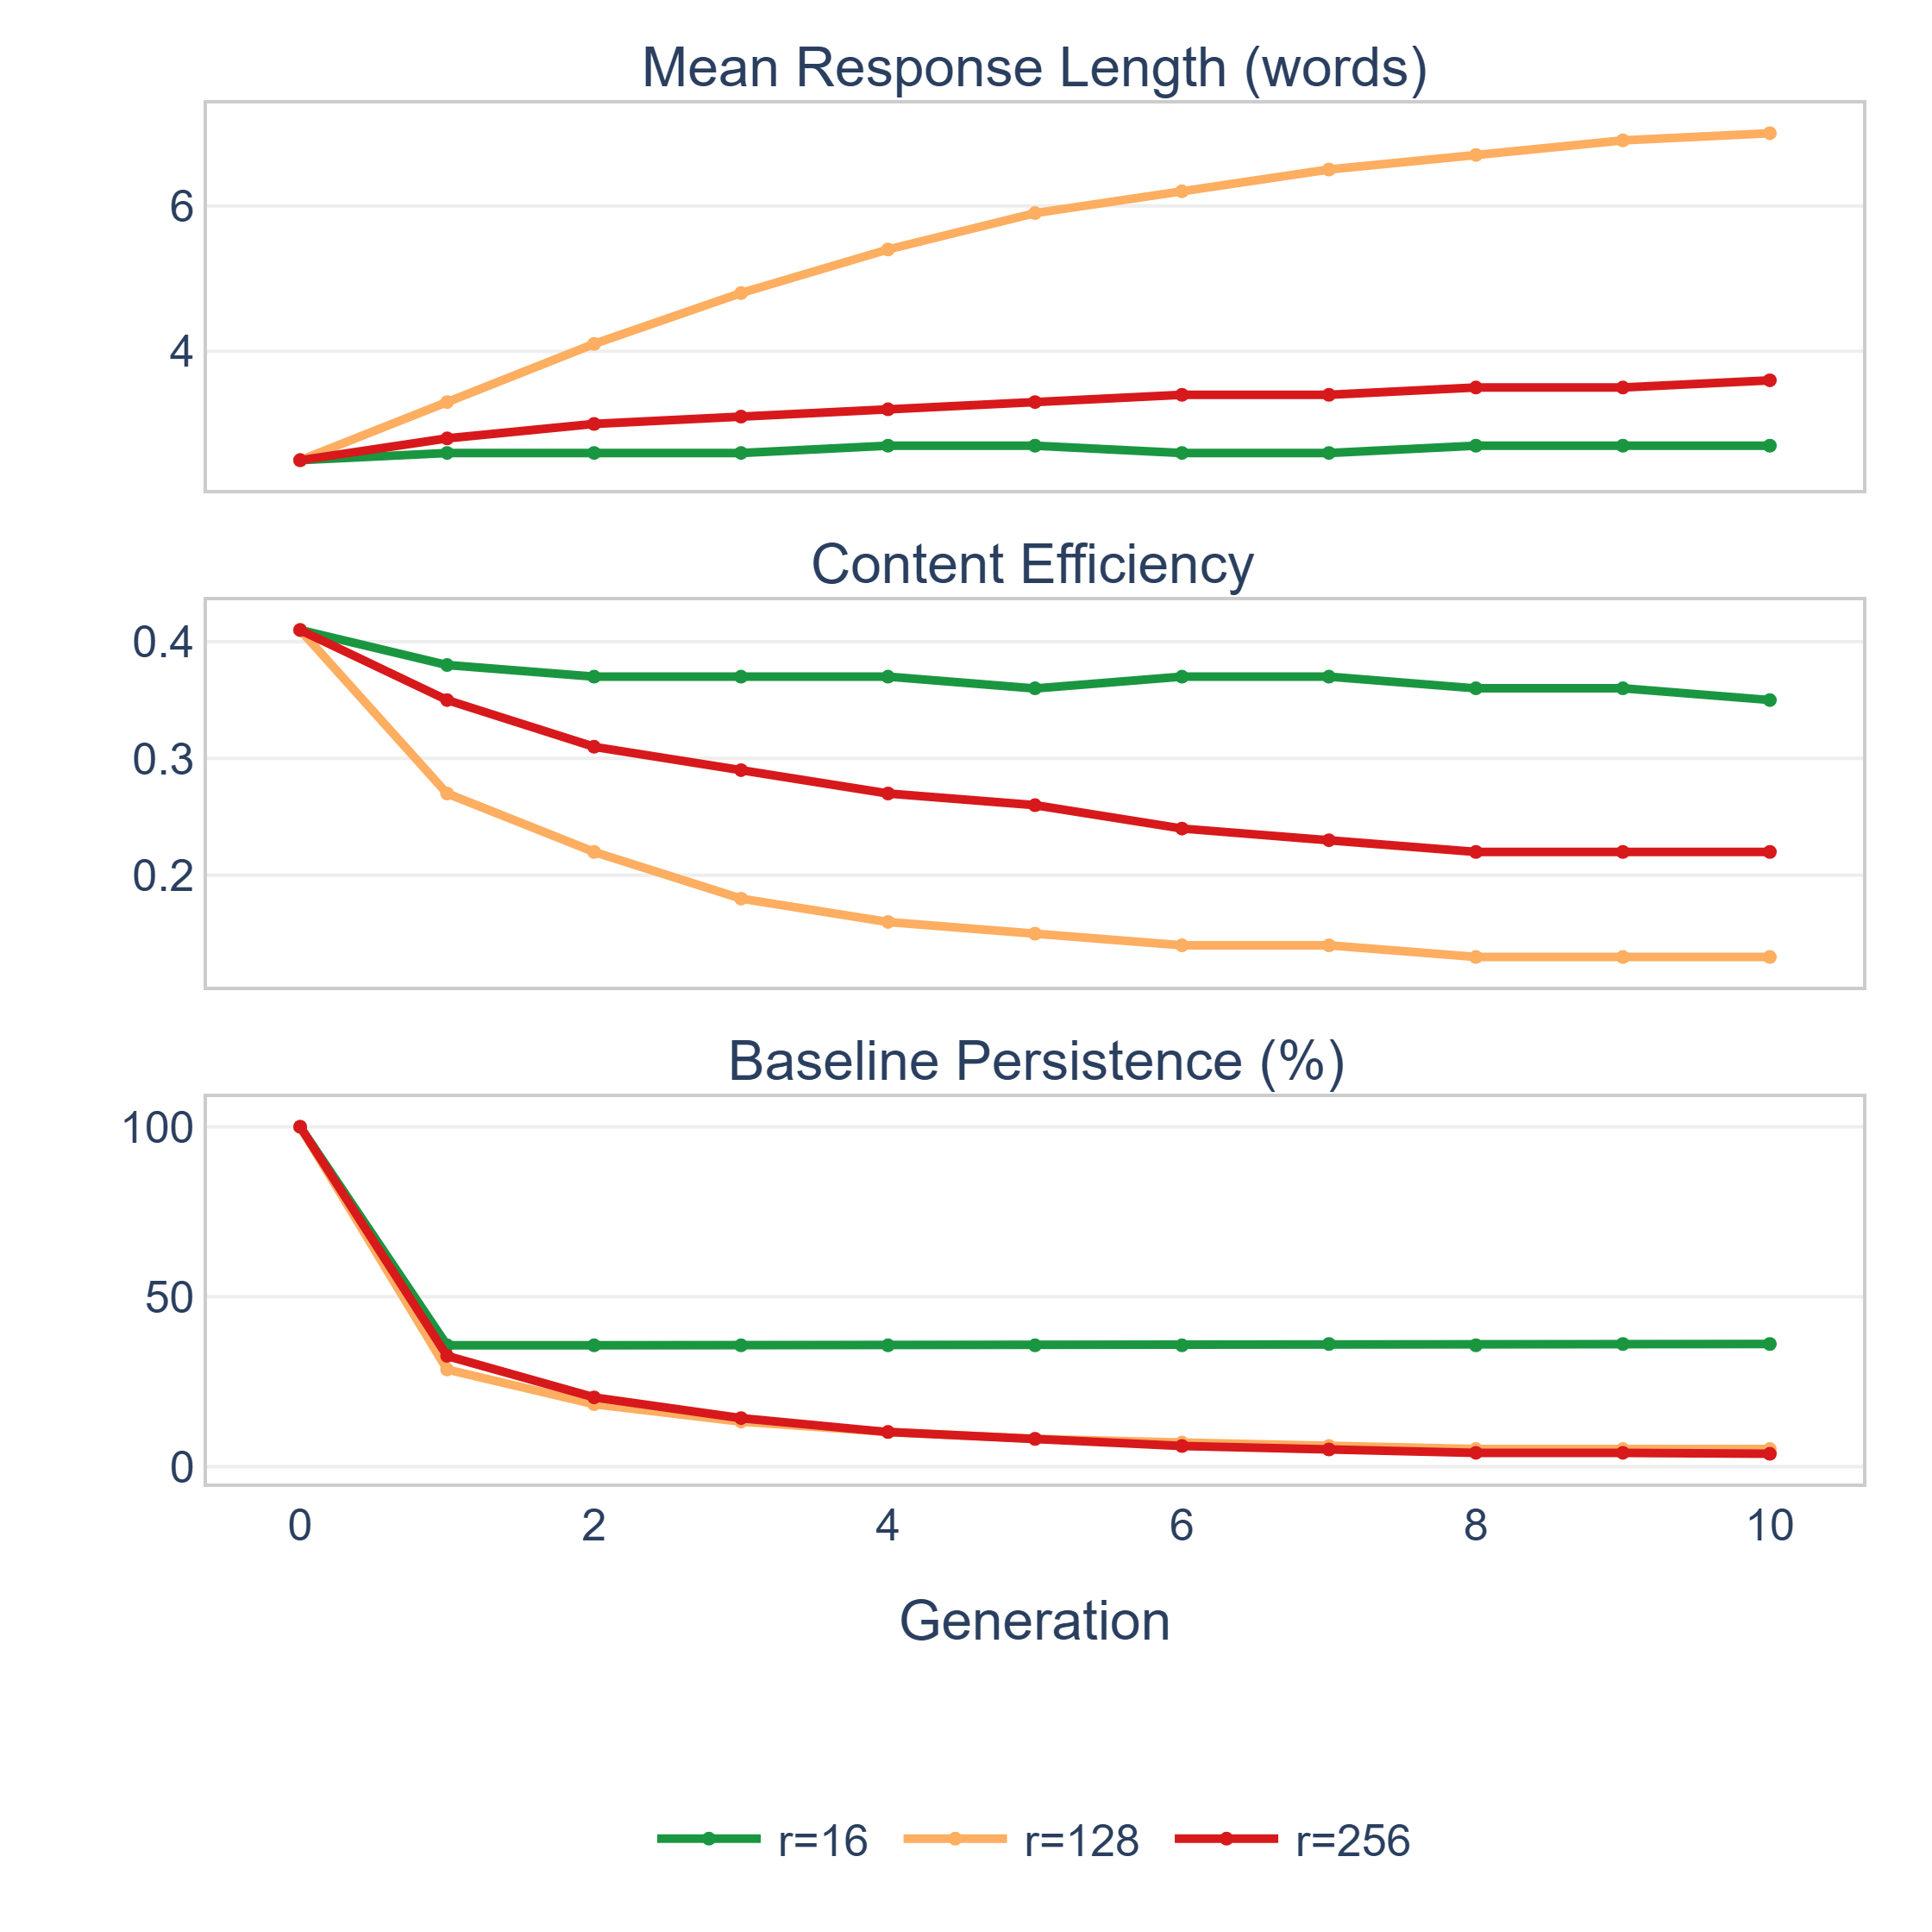
\includegraphics[width=0.95\columnwidth]{figs/final/fig5_distributional.png}
  \caption{Distributional diagnostics over ten recursive generations for three
  representative Qwen configurations. (a)~Mean response length, (b)~baseline
  response persistence, (c)~content efficiency. All three metrics diverge for
  $r=128$ and $r=256$ while remaining stable for $r=16$; the $r=128$
  configuration is notable for strong distributional drift despite bounded
  factual retention.}\label{fig:distributional}
\end{figure}

The figure reveals three distinct patterns. For $r=16$ (homeostatic), all three
metrics remain flat, confirming that the output stream is stable. For $r=256$
(degradative), all metrics diverge from baseline simultaneously with retention
loss. The most informative case is $r=128$: response length doubles and content
efficiency collapses to one-third of its initial value, yet factual retention
remains above 89\%, demonstrating that distributional degradation can proceed
substantially before factual accuracy signals any problem.

To examine whether output drift precedes factual loss, we computed cross-lag
correlations between mean response length at generation~$t$ and retention at
generation~$t{+}1$. The raw Pearson correlation in the degradative regime is
strong ($\rho = -0.965$), but robustness analyses substantially attenuate this
association. After conditioning on shared temporal trend (partial correlation),
the coefficient drops to $-0.22$. First-difference analysis yields $-0.43$, and
the reverse-lag correlation is of comparable magnitude, indicating a
bidirectional association rather than clear temporal precedence.

Output drift is therefore interpreted as a co-symptom of the same underlying
high-pressure process, rather than a demonstrated causal antecedent of factual
loss. Output drift remains valuable as a diagnostic signature: it is
consistently present in degradative and distributionally degraded configurations,
consistently absent in stable configurations, and can appear even when factual
retention remains bounded, as illustrated by the $r=128$ configuration.
Determining the causal relationship between output-distribution changes and
factual degradation remains an open question.

The next section tests whether the third component of effective training
pressure, synthetic data exposure, can shift the system back toward homeostasis
at the regime boundary.

\subsection{Synthetic exposure interventions}\label{sec:res_intervention}

The preceding sections established that update capacity and perturbation
magnitude each govern the regime transition. This section tests the third
component of effective training pressure: whether reducing synthetic data
exposure can shift the system back from a degradative to a near-homeostatic
configuration. The primary evidence comes from the two pre-registered
dose--response experiments described in Section~\ref{sec:intervention}:
B7 on Qwen $r=256$ ($n=5$ paired seeds, $K_0=78$) and G2 on Gemma~3 $r=10$
($n=3$ paired seeds, $K_{0,\mathrm{G2}}=44$).

\rev{Table~\ref{tab:interventions} reports $K_0$ retention and the gain over
the 0\% within-pipeline baseline for each dose level on Qwen $r=256$.}

\begin{table}[width=.95\linewidth,cols=5,pos=htbp]
\caption{\rev{Dose--response on Qwen $r=256$ ($|K_0|=78$, $n=5$ paired seeds per
dose). Retention and gain ($\Delta$) relative to the 0\% within-pipeline
baseline at Gen5 and Gen10.}}\label{tab:interventions}
\begin{tabular*}{\tblwidth}{@{} llrrrl@{} }
\toprule
\rev{Dose} & \rev{Ret.\ (Gen5)} & \rev{$\Delta$ Gen5} & \rev{Ret.\ (Gen10)} & \rev{$\Delta$ Gen10} & \rev{$N_\mathrm{seeds}$} \\
\midrule
0\%  & 84.0\% & ---             & 79.1\% & ---             & 5 \\
10\% & 89.0\% & $+5.0$\,pp      & 81.6\% & $+2.4$\,pp      & 5 \\
25\% & 89.2\% & $+5.3$\,pp      & 84.6\% & $+5.5$\,pp      & 5 \\
50\% & 89.7\% & $+5.7$\,pp      & 88.9\% & $+9.8$\,pp      & 5 \\
\bottomrule
\end{tabular*}
\end{table}

% [v4-revision: C1-C5 pilot archived in replication repository; not used in primary estimates]

\rev{\textbf{Qwen dose--response (B7).}
A pre-registered dose--response experiment on Qwen $r=256$ (five paired seeds;
protocol registered as \texttt{a916ebf} before any run) shows that the
Gen~10 benefit is graded: $+2.4$\,pp at 10\% removal ($p = 0.002$, $n=5$),
$+5.5$\,pp at 25\% (95\%~CI $[0.4, 10.5]$, $p = 0.039$), and
$+9.8$\,pp at 50\% (95\%~CI $[6.9, 12.8]$, $p = 0.0008$). At Gen~5, the
gains are smaller and more uniform ($+5.0$, $+5.3$, $+5.7$\,pp;
paired $t$-test $p = 0.002$, $0.014$, $0.002$). A 50\% reduction
effectively arrests progressive loss: the Gen~5$\to$10 slope is
$-0.14$\,pp/generation versus $-0.96$\,pp/generation at 0\%, shifting the
system from the degradative to the bounded regime by the criterion of
Section~\ref{sec:res_capacity}.

The pre-registered prediction that 50\% removal would match halving the
learning rate (from $\eta = 10^{-5}$ to $5\times 10^{-6}$) was numerically similar:
Gen~5 retention at dose~$= 50\%$ is $89.7\%$ versus $90.2\%$ at
$\eta = 5\times 10^{-6}$ (mean over three seeds; Gen~10 difference
$+0.4$\,pp, 90\%~CI $[-0.8, 1.6]$). The mechanism (whether update budget
or data composition) was not established; a steps-matched control was
inconclusive at $n = 3$.

The original C1--C5 pilot compared non-identical evaluation pipelines;
when C1 and C5 are re-run under an identical pipeline and paired seeds,
the approximate $5\%$ downsampling effect is $+1.9$\,pp ($n=3$, not
statistically distinguishable from zero). We therefore exclude the
original pilot from the primary effect estimate; those results are
archived in the replication repository (Section~\ref{app:repo}).}

Figure~\ref{fig:interventions} visualizes the retention and effect-size
comparison across conditions.

\rev{\begin{figure}[tp]
  \centering
  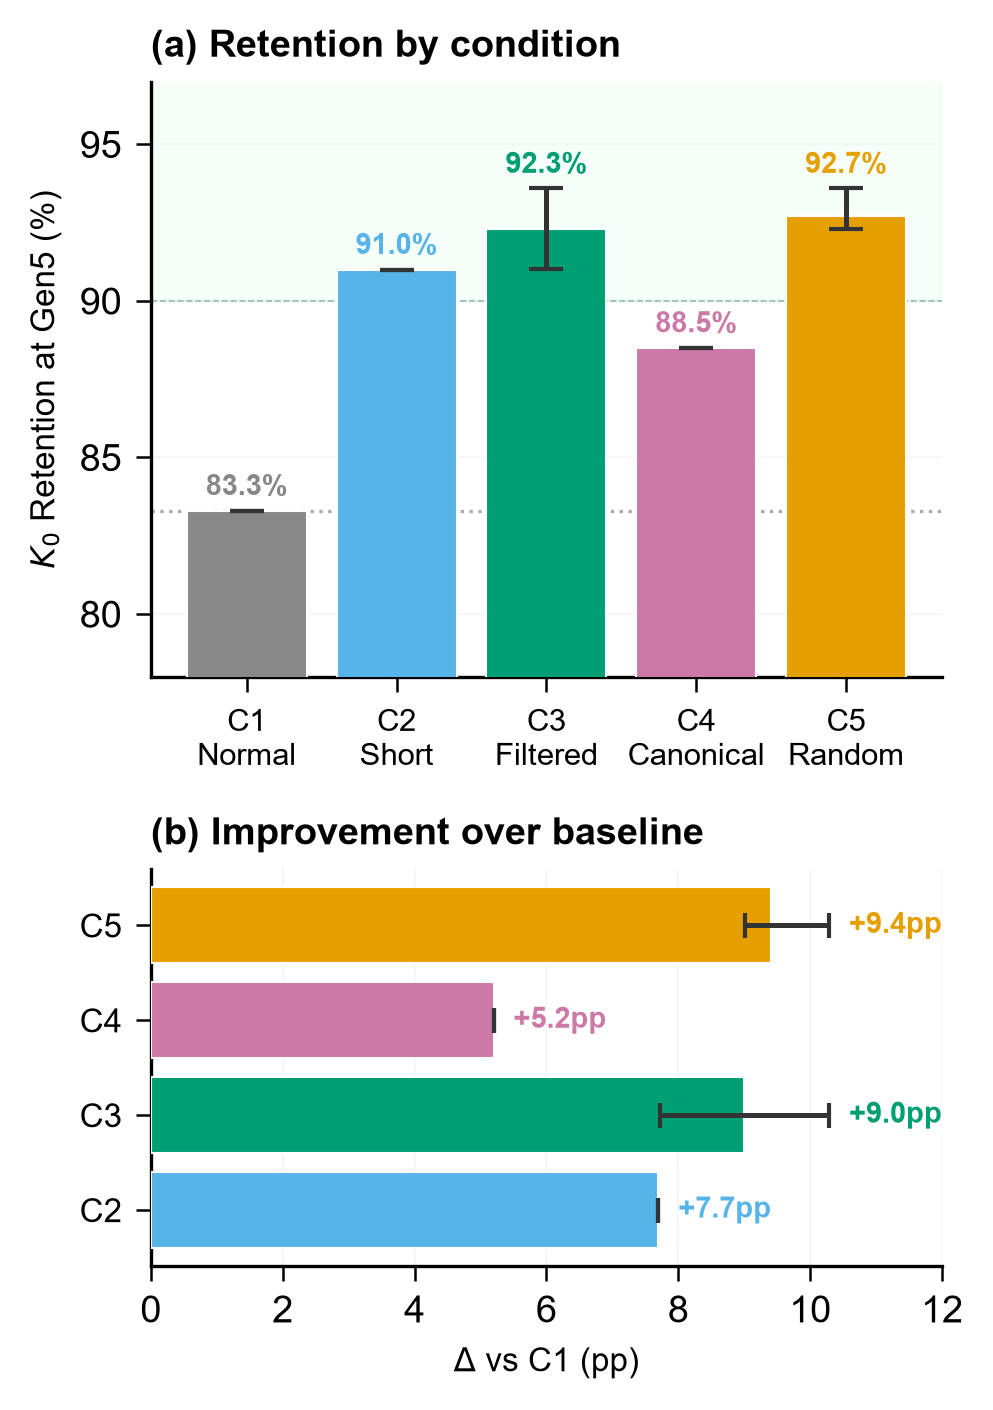
\includegraphics[width=0.95\columnwidth]{figs/scratch/fig_interventions.png}
  \caption{Exploratory pilot (C1--C5) on Qwen $r=256$ at Gen5, included for
  transparency. These results use a different evaluation pipeline from the
  primary dose--response experiments (B7/G2) and are not used in the primary
  effect estimates. (a)~$K_0$ retention by condition. (b)~Retention improvement
  relative to the corresponding unmodified arm; error bars reflect the range across three seeds or
  masks.}\label{fig:interventions}
\end{figure}}

\rev{These results demonstrate that the Qwen $r=256$ configuration responds to
graded exposure reduction: a 50\% reduction arrests progressive loss and shifts
the system to the bounded regime, whereas a 10\% reduction does not. This
graded dose--response is confirmed on a second backbone (Gemma~3 G2, see below).
The sensitivity is tested only at the configurations evaluated here and should
not be interpreted as a universal property of recursive fine-tuning.}

\rev{\textbf{Dose--response replication on Gemma~3.}
A parallel pre-registered dose--response experiment on Gemma~3 at $r=10$
(G2, three seeds, four doses) confirms that the exposure effect generalises
to a second backbone. At the unmodified baseline (dose~$=0\%$), Gemma~3 at
$r=10$ shows progressive degradation ($\GtwoMtenZero\%\pm\GtwoSDtenZero$~pp
Gen10, slope $\GtwoSlopeZero$~pp/gen). Reducing exposure by 10\%, 25\%, and
50\% raises Gen10 retention by $\GtwoDeltatenTen$~pp
($p=\GtwoPtenTen$), $\GtwoDeltatenTfive$~pp ($p=\GtwoPtenTfive$), and
$\GtwoDeltatenFifty$~pp (95\,\% CI $[\GtwoCItenLoFifty, \GtwoCItenHiFifty]$,
$p=\GtwoPtenFifty$), respectively ($n=3$ paired seeds per dose).
At dose~$=50\%$, the slope is $\GtwoSlopeFifty$~pp/gen, indicating
near-arrest of progressive loss.}
\rev{The absolute gain at dose~$=50\%$ Gen10 is larger for Gemma~3 G2
($\GtwoDeltatenFifty$~pp, $K_{0,\mathrm{G2}}{=}44$) than for Qwen B7
($\BsevenDeltatenFifty$~pp, $K_0{=}78$). The two experiments used different
backbones, different evaluation set sizes, and different baseline retention
levels; effective rank is not portable across architectures
(Section~\ref{sec:res_backbone}), so we report the gains within each
protocol without inferring which backbone operated at higher relative
pressure.}

\rev{\begin{figure}[tp]
  \centering
  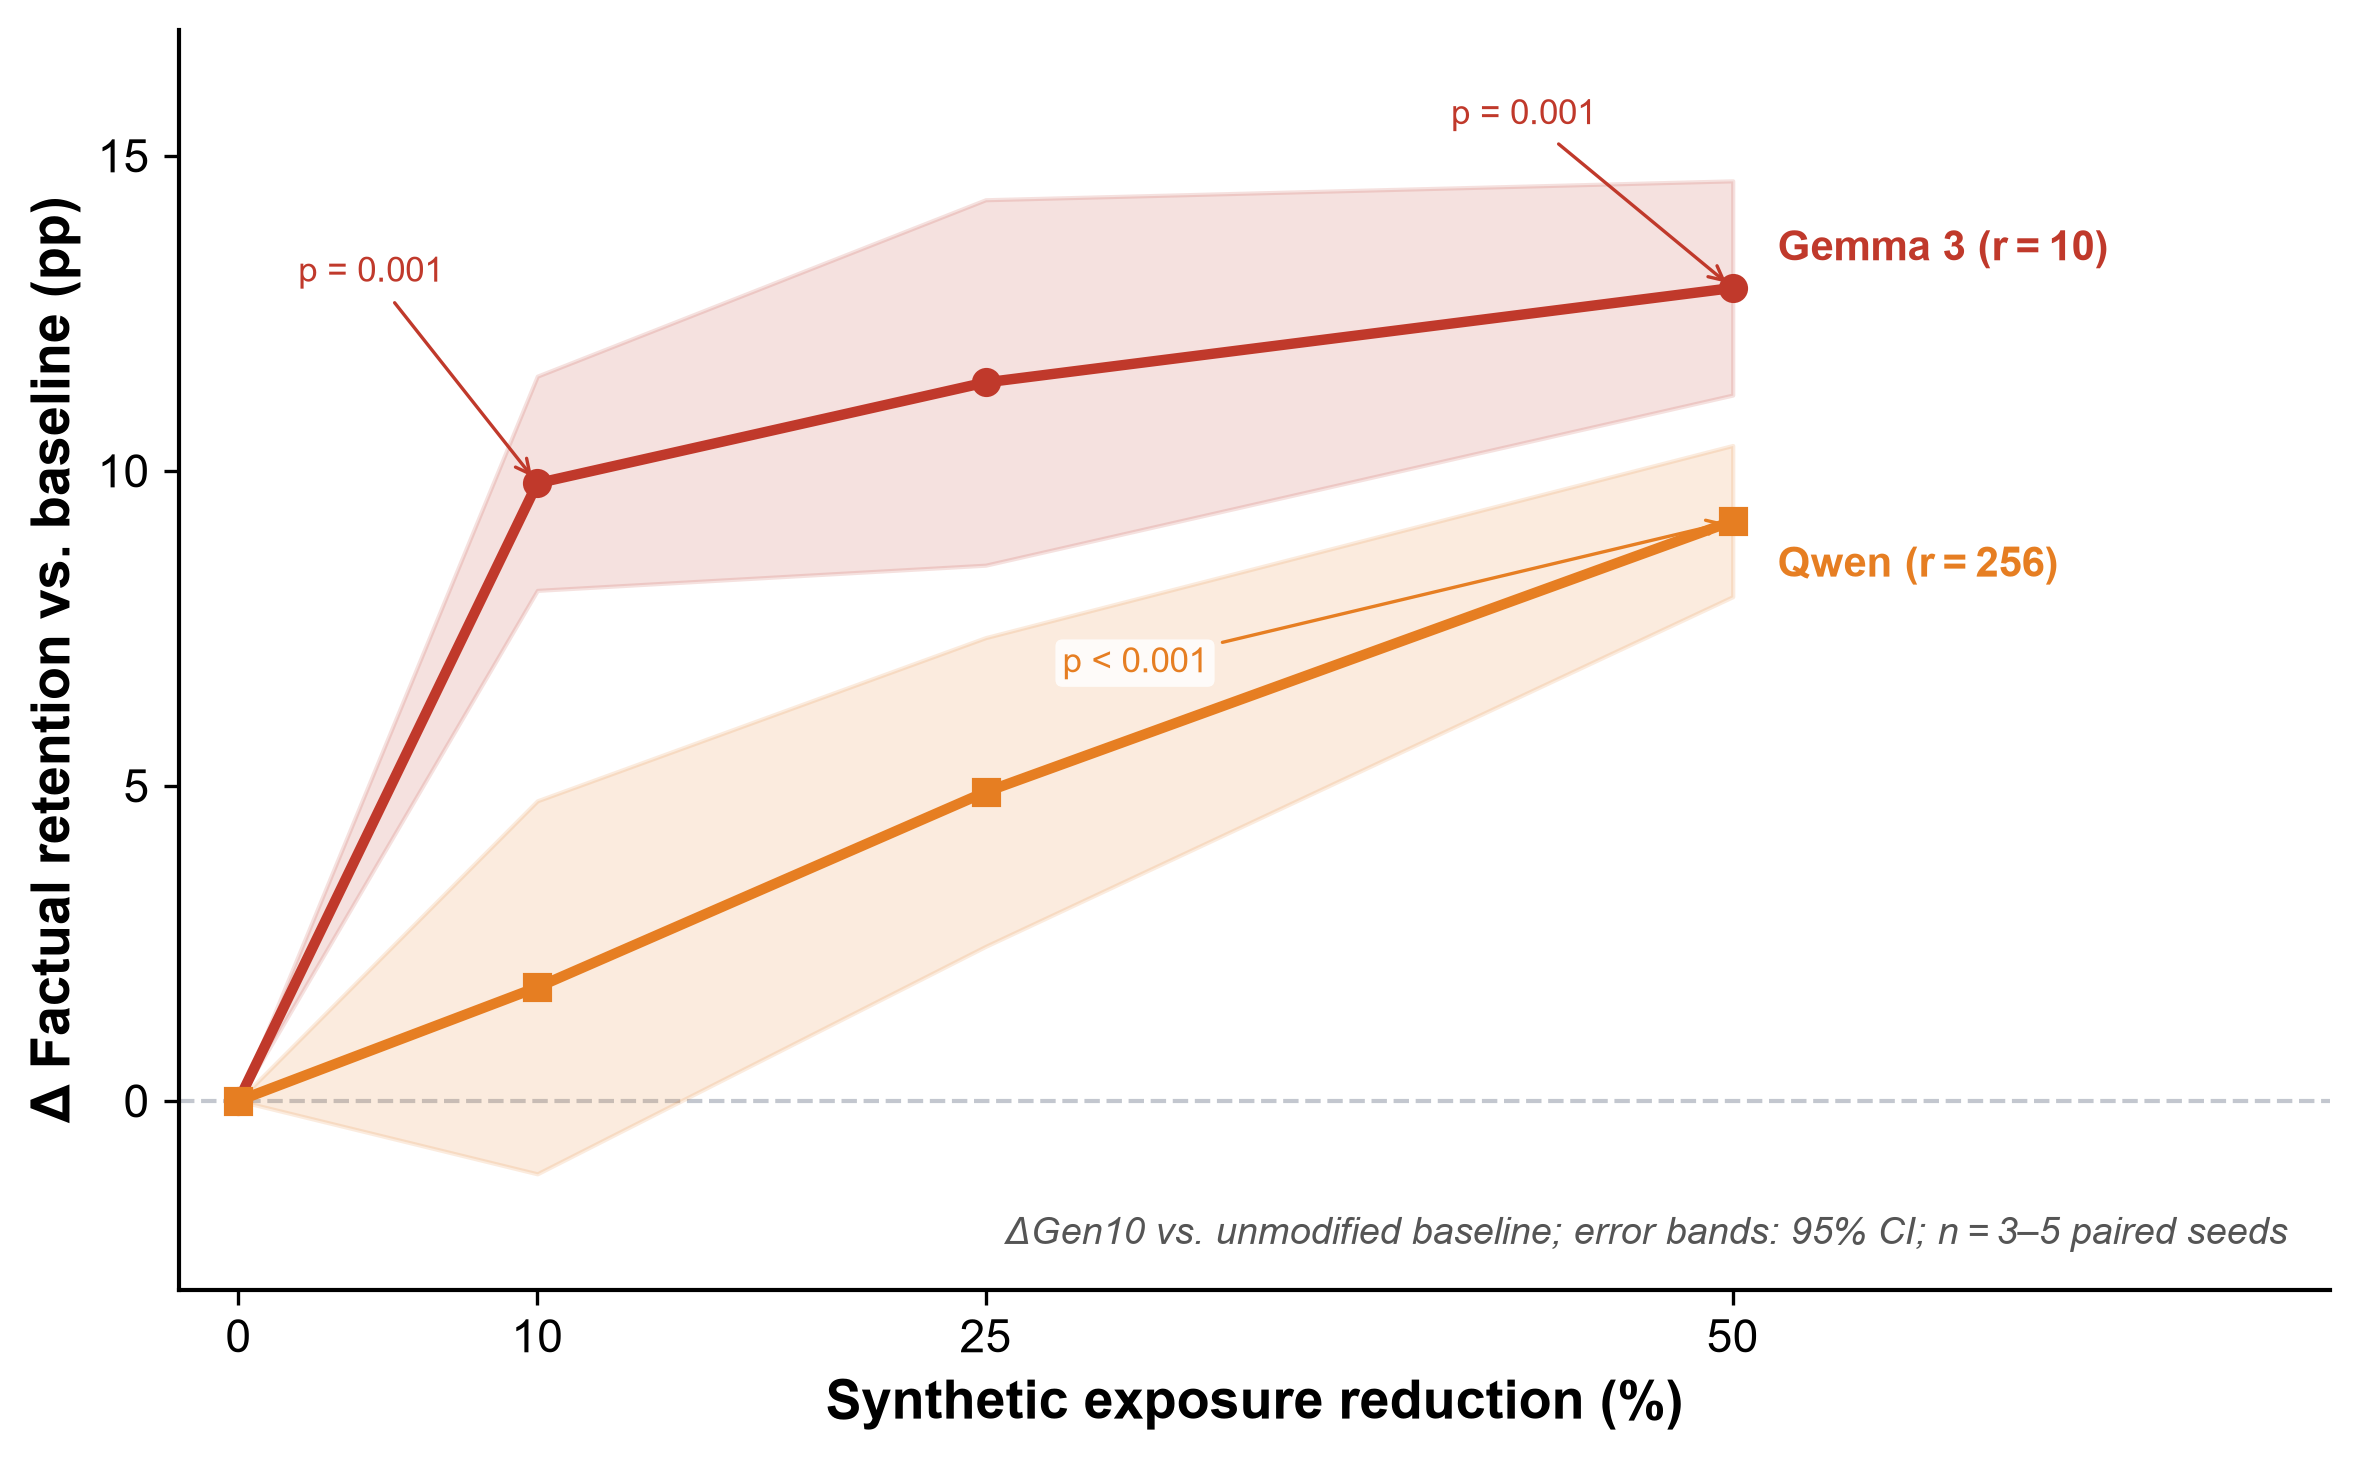
\includegraphics[width=0.95\columnwidth]{figs/final/fig9_dose_response.png}
  \caption{Dose--response of synthetic exposure reduction on factual retention
  across two backbones (Gen10, $K_0$-conditioned). Each curve shows the mean
  improvement ($\Delta$pp) over the respective unmodified baseline as the
  fraction of synthetic training examples removed increases from 0\% to 50\%.
  Red circles: Gemma~3~1B at $r=10$ ($n=3$ paired seeds; $K_{0,\mathrm{G2}}=44$).
  Orange squares: Qwen~2.5~1.5B at $r=256$ ($n=5$ paired seeds; $K_0=78$).
  Shaded bands: 95\,\% confidence intervals from paired $t$-tests.
  The absolute gain is larger for Gemma~3 G2 ($K_{0,\mathrm{G2}}{=}44$)
  than for Qwen B7 ($K_0{=}78$); effective rank is not portable across
  architectures, so the two curves are reported within their respective
  protocols rather than as a cross-backbone pressure comparison.
  Dashed horizontal line: no change ($\Delta=0$~pp).}\label{fig:dose_response_crossbackbone}
\end{figure}}

Taken together, the intervention experiments show that the degradative regime is
reversible under the evaluated conditions. Adjusting synthetic exposure restores
near-homeostatic behavior in the \rev{lowest-pressure degradative configuration tested}, complementing the
capacity and perturbation results presented in the preceding sections. We note
that verification-based approaches \citep{yi2025} represent an orthogonal
mitigation axis (filtering by quality rather than quantity); our exposure
reduction experiments test boundary sensitivity rather than proposing a
competing mitigation pipeline.

Collectively, the five experimental axes establish that recursive stability
under PEFT is governed by a multidimensional pressure landscape: update
capacity, perturbation magnitude, and synthetic exposure each independently
shift the system between regimes, these axes interact rather than operate in
isolation, and the regime boundary is backbone-dependent. The following section
interprets these findings in the context of prior work.

% ============================================================
% 4.6  EXPERIMENTAL CONTROLS (G3, G4, G5)
% ============================================================
\subsection{Experimental controls and prospective index}\label{sec:res_controls}

\rev{\textbf{Quantization control (G3).}
All main QLoRA experiments use 4-bit NormalFloat (NF4) quantization of the base
weights. To verify that the regime classification is not an artifact of NF4, we
re-ran the same protocol on Qwen using standard bf16 precision and no base-weight
quantization (G3, three seeds at each of $r=16$ and $r=256$). At $r=16$, bf16
yields $97.4\%$ Gen10, a difference of $\GthreeDeltatenSixteen$~pp from the NF4
baseline; at $r=256$ the difference is $\GthreeDeltatenTwoFiveSix$~pp.
The G1 (NF4) and G3 (bf16) runs produced identical aggregate retention counts
for the matched seeds at $r=256$; run-level provenance and item-level outputs
are audited separately before interpreting this agreement as evidence about
quantization. The regime classification at both ranks is consistent across
precision settings, but a causal conclusion about quantization awaits full
provenance audit.}

\rev{\textbf{Data-order control (G4).}
To isolate seed variance from data-order variance, G4 replicates the Qwen
$r=256$ protocol with three new shuffle seeds (42/101/202). Gen10 retention
values are $82.1\%$, $78.2\%$, and $80.8\%$, yielding a G4 mean of $80.4\%\pm2.0$~pp.
A bilateral permutation test comparing G1 and G4 gives $p=\GfourPorder$, indicating
no detectable signal beyond seed-to-seed variance. Because G4 varies both data
order and random seed simultaneously, $p=\GfourPorder$ does not isolate the
effect of order alone; it establishes that the combined variance is
statistically indistinguishable from G1. Combining G1$+$G4 gives a six-seed
Gen10 estimate of $\GoneFourMten\%\pm\GoneFourSDten$~pp
(95\,\% CI $[\GoneFourCItenLo, \GoneFourCItenHi]$).}

\rev{\textbf{Prospective rank$\times$learning-rate probe (G5).}
As a prospective test of whether the regime ordering generalises to unseen
rank$\times$learning-rate configurations, we pre-registered three cells on
Qwen~2.5~1.5B with a single seed (seed~15, five generations): a low-pressure
cell ($r=128$, $\eta=5\times10^{-6}$), a high-pressure cell ($r=128$,
$\eta=2\times10^{-5}$), and an intermediate cell ($r=32$, $\eta=2\times10^{-5}$).
The pre-registered classification predicted Homeostatic, Degradative, and
Bounded respectively, based on the rank$\times$LR grid established in
\S\ref{sec:res_capacity}.
The low-pressure cell returned $\GfiveRonetwoetightLRlow\%$ at Gen5
(Homeostatic, \textbf{confirmed}); the high-pressure cell returned
$\GfiveRonetwoetightLRhigh\%$ (Bounded, \textbf{not confirmed}; predicted
Degradative); and the intermediate cell returned $\GfiveRthreytwoLRhigh\%$
(Bounded, \textbf{confirmed}).
We do not report an operational pressure index $\Pi$ for G5: the effective rank
of each adapter was measured (mean $\mathrm{erank}\approx51$ for $r=128$,
$\approx16$ for $r=32$), but the pre-specification did not fix a threshold on
$\Pi$, and the three cells were selected by nominal rank and learning rate, not
by $\Pi$ value. One of the three pre-specified regime classifications was not
met; G5 is therefore exploratory evidence for the ordering, not a confirmatory
test of the full classification scheme.
All three cells used a single seed; the prospective result is therefore exploratory.}
\section{Discussion}\label{sec:discussion}

The preceding results identify consistent patterns in how recursive synthetic
fine-tuning responds to changes in update capacity, perturbation magnitude, and
synthetic exposure. This section interprets these findings in the context of
prior work, examines what they imply for the understanding and management of
recursive training systems, and discusses the limitations of the present study.
The discussion is organized around four themes: the interpretation of effective
training pressure as an organizing framework
(Section~\ref{sec:disc_pressure}), the relationship between the present findings
and the model-collapse literature (Section~\ref{sec:disc_literature}), the
diagnostic role of output-distribution changes (Section~\ref{sec:disc_drift}),
and the practical implications for the design and monitoring of recursive
training pipelines (Section~\ref{sec:disc_practical}).

\subsection{Effective training pressure as framework}\label{sec:disc_pressure}

\begin{figure*}[t]
  \centering
  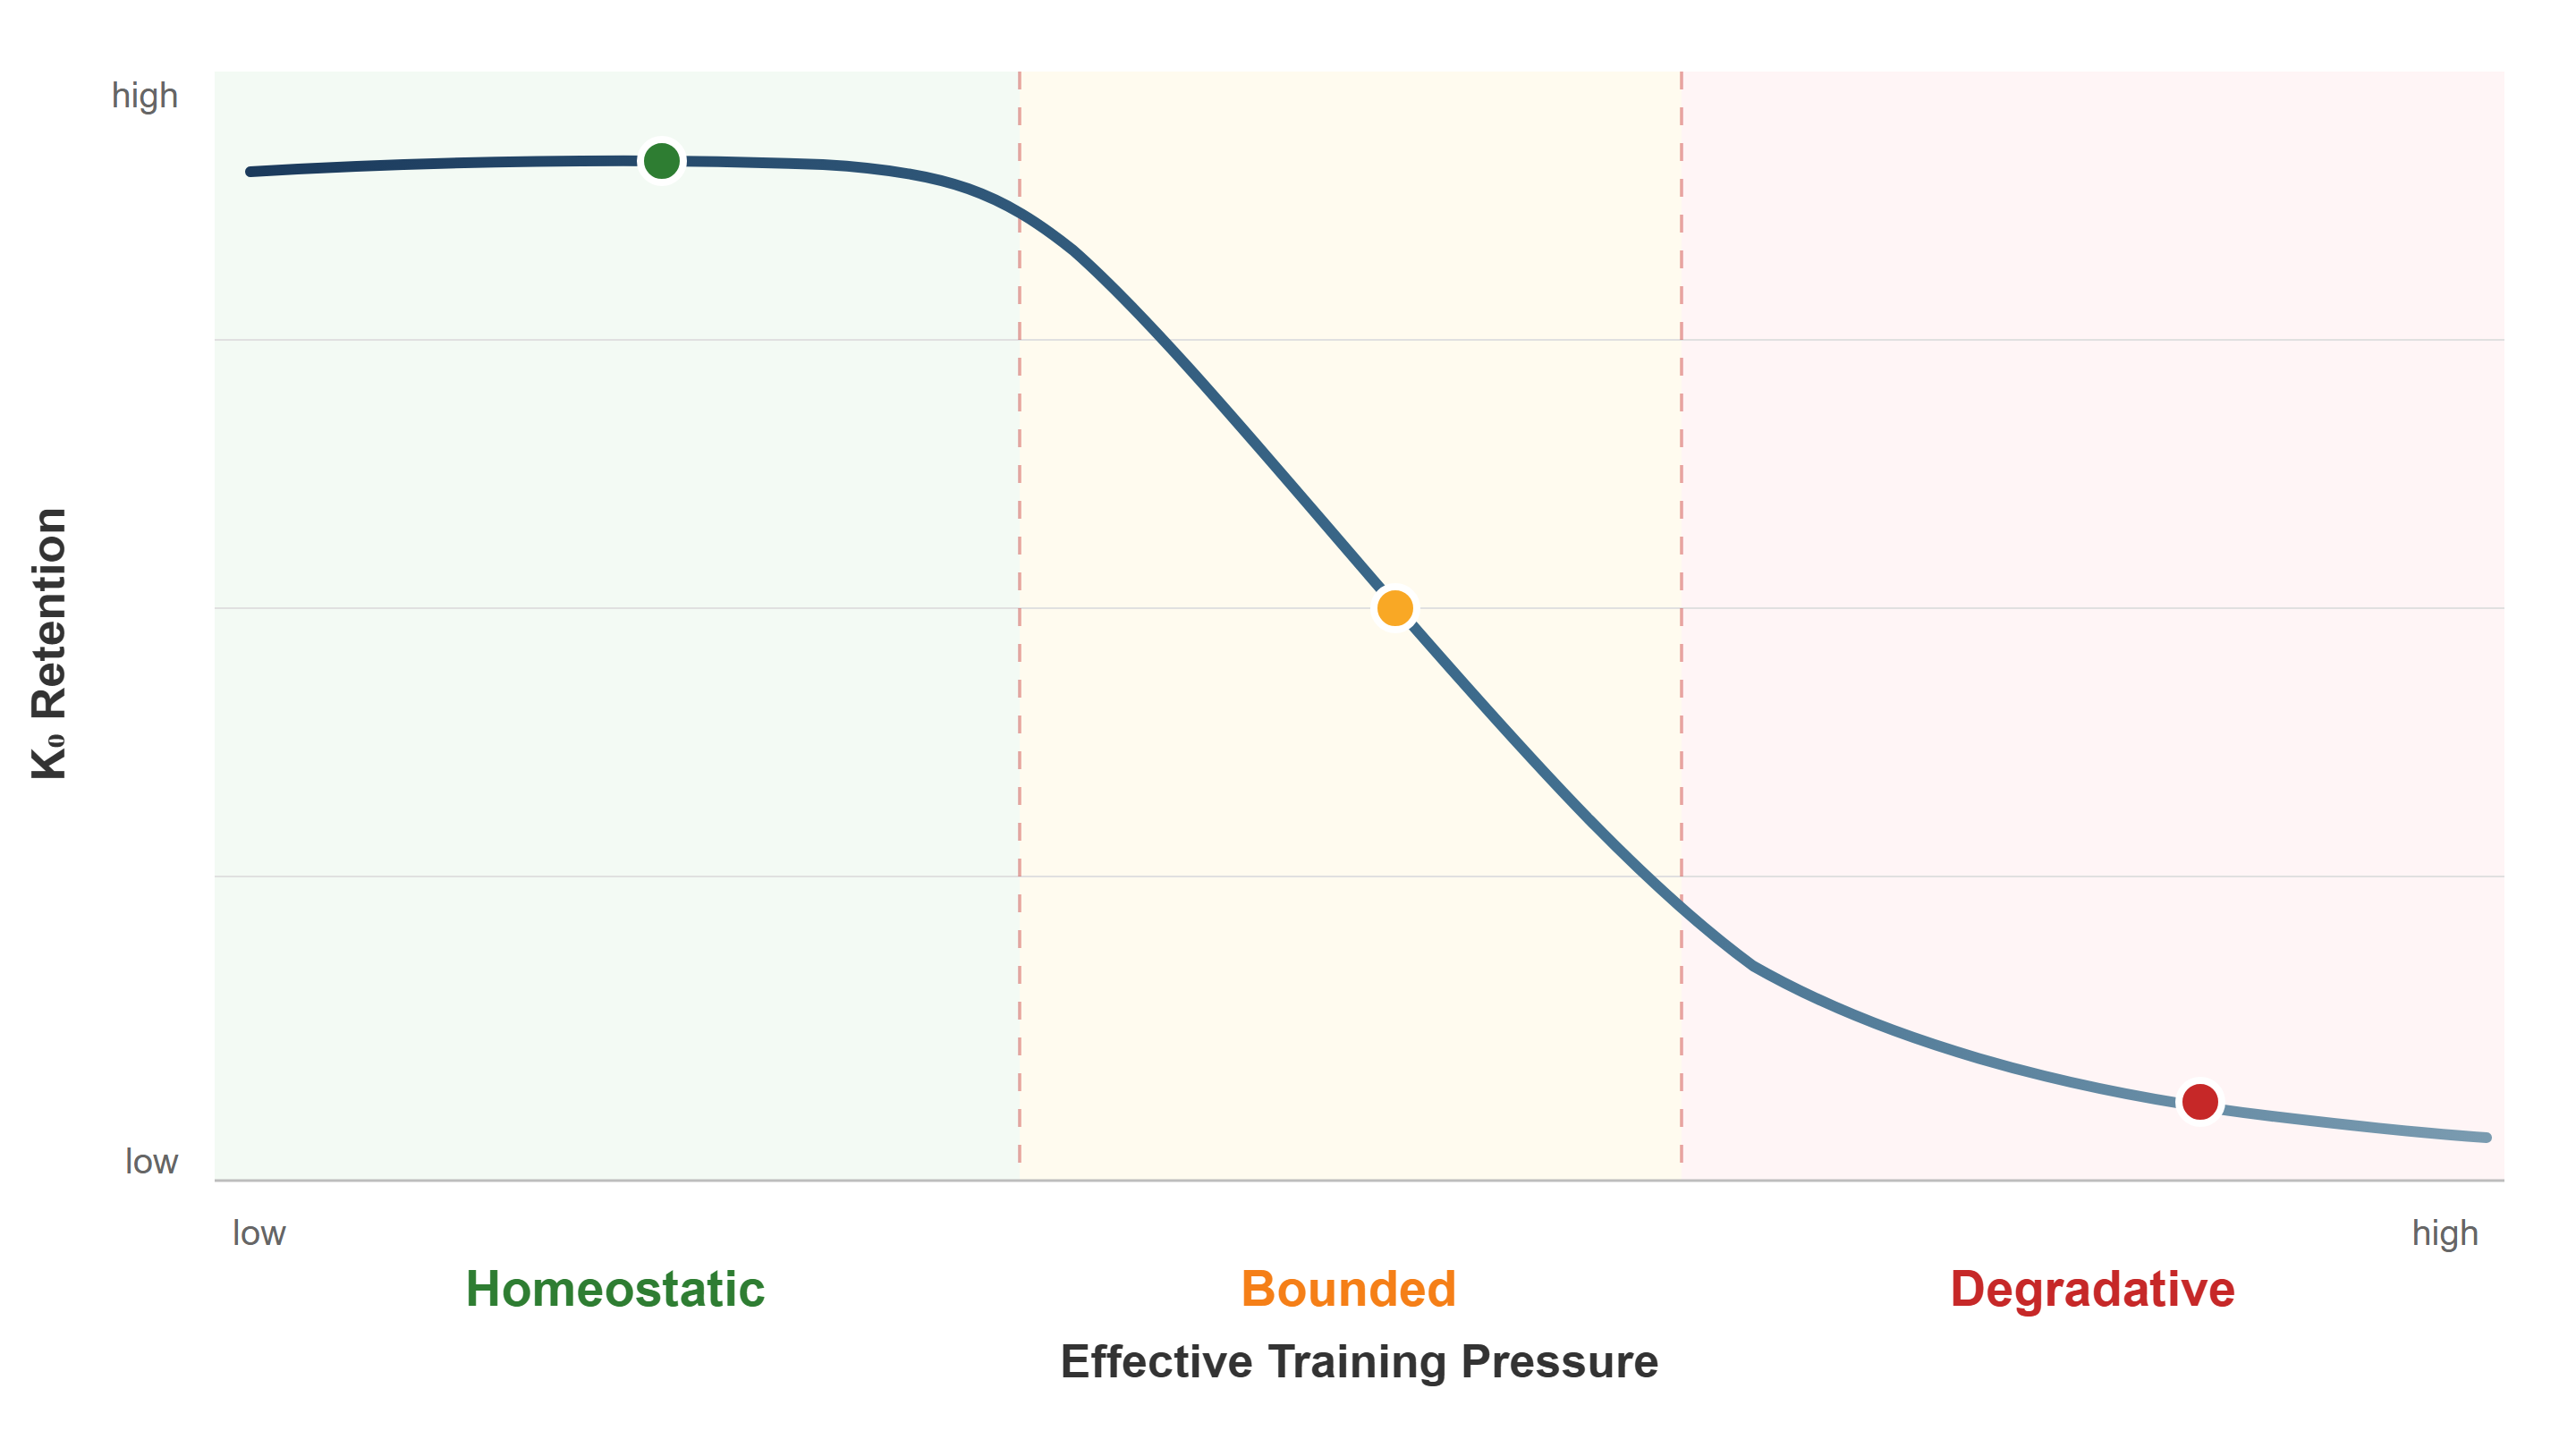
\includegraphics[width=0.75\textwidth]{figs/scratch/fig_etp_framework.png}
  \caption{Pressure-response relationship guiding recursive fine-tuning
  stability. Factual retention transitions through three regimes as effective
  training pressure increases. Dashed lines mark backbone-dependent boundaries;
  the transition is abrupt and its location varies by roughly an order of
  magnitude across architectures.}\label{fig:etp}
\end{figure*}

The results presented in Section~\ref{sec:results} converge on a consistent
empirical pattern: recursive factual degradation is not observed uniformly
across recursive synthetic fine-tuning, but instead emerges only when the
training process operates above a backbone-dependent pressure threshold. Three
independently manipulated variables, adapter rank, learning rate, and synthetic
exposure, each shift the system between homeostatic and degradative behavior.
The convergence of these independent manipulations is the primary empirical
motivation for treating them as manifestations of a common organizing principle.

The framework is empirical rather than theoretical. We do not propose a
closed-form expression that combines rank, learning rate, and exposure into a
single scalar predictor. Instead, the experiments reveal that each variable independently
controls the same qualitative transition. \rev{The transition is abrupt within the tested
parameter grid: at Gen~10, a 50\% reduction in synthetic exposure arrests progressive
loss ($-0.14$\,pp/generation), whereas a 10\% reduction does not
($-1.48$\,pp/generation). This abruptness is consistent with the system operating
near a regime boundary, though the present experiments do not establish a
precise threshold value that will generalise to other settings.}

\rev{The contribution is the existence and reproducibility of this
abrupt transition within the tested grid, not the numerical threshold itself.} The present work does not claim that the
specific effective-rank values at which regimes change will generalize to
arbitrary models or tasks. What appears to generalize is the qualitative
structure: a pressure-dependent boundary separating stable from degradative
recursive behavior, controllable through multiple axes.

The rank $\times$ learning-rate joint-dependence experiment
(Table~\ref{tab:ranklr}) further demonstrates that these axes are not
independent: different combinations of rank and learning rate produce similar
recursive outcomes, indicating that the regime depends jointly on both variables.
This result strengthens the interpretation of effective training pressure as a
multidimensional control landscape rather than a collection of separable
single-variable effects. Beyond the interaction itself, two additional
convergences support this interpretation:
the transition boundary induced by each axis shares the same qualitative
signature (abrupt rather than gradual), and the same distributional drift patterns
accompany degradation regardless of which axis crosses the threshold. These
convergences would be coincidental under a model of three independent failure
modes, but are naturally explained by a shared underlying sensitivity to the
magnitude of per-generation parameter perturbation. Developing a quantitative
formulation that combines update capacity, perturbation magnitude, and exposure
into a single predictive scalar remains an important direction for future work.

Table~\ref{tab:evidence} summarizes how each component of the framework is
supported by independent experimental evidence.

\begin{table}[tp]
\caption{Evidence matrix: mapping framework components to supporting
experiments.}\label{tab:evidence}
\footnotesize
\renewcommand{\arraystretch}{1.4}
\begin{tabularx}{\columnwidth}{@{}lX@{}}
\toprule
\textbf{Observation} & \textbf{Supporting evidence} \\
\midrule
Rank governs transition & Rank sweep, 6 values, $N{=}3$ at $r{=}16$, $r{=}256$ \\
\addlinespace
Magnitude governs transition & FFT LR sweep, 4 values \\
\addlinespace
\rev{Exposure reduces pressure} & \rev{Dose--response 0--50\%, $N{=}5$ seeds (pre-registered)} \\
\addlinespace
Threshold is backbone-dependent & Qwen vs Gemma~3 ($10{\times}$ gap) \\
\addlinespace
Drift accompanies degradation & 5 distribution metrics \\
\addlinespace
\rev{Transition is abrupt within tested grid} & \rev{Dose--response plateau at Gen~5; graded at Gen~10} \\
\addlinespace
Capacity $\times$ magnitude \rev{joint dependence} & Rank $\times$ LR matrix ($3{\times}3$) \\
\addlinespace
Generalizes cross-backbone & Gemma~3 (N=5) + E2B dose-response \\
\bottomrule
\end{tabularx}
\end{table}

Two features of this framework merit emphasis. First, the threshold is
backbone-dependent: Gemma~3 transitions at effective rank 3--6, while Qwen
remains outside the degradative regime up to effective rank ${\sim}$50. No simple normalization by architectural
parameters (hidden dimension, depth, head count) aligned these thresholds. This
likely reflects properties of the pretrained backbone not captured by simple
architectural dimensions. Second, the framework does not assume that the three
pressure components are interchangeable or commensurable. Rank and learning rate
operate through different mechanisms (subspace dimensionality versus step size),
and synthetic exposure operates on the data stream rather than the update
itself. Their shared effect on the regime transition is the empirical
observation that motivates the framework, not a theoretical prediction.

\subsection{Relation to recursive-training literature}\label{sec:disc_literature}

The model-collapse literature has established that recursive training on
synthetic data can produce irreversible degradation under full fine-tuning
\citep{shumailov2024} and that expected loss increases linearly with any
nonzero fraction of synthetic data \citep{dohmatob2025}. Our results do not
contradict these findings. Rather, they help localize the experimental
conditions under which qualitatively similar degradation emerges in our
recursive fine-tuning setting: the degradative configurations ($r=256$ on Qwen,
$r \geq 16$ on Gemma~3, FFT at high learning rates) are qualitatively
consistent with the collapse dynamics these works describe.

The contribution of the present work is locating where, in the space of
practical PEFT configurations, the transition between bounded and degradative
behavior occurs. \citet{biderman2024} observed that LoRA ``learns less and
forgets less'' relative to full fine-tuning. Empirical studies of catastrophic
forgetting in LLMs during continual fine-tuning \citep{luo2023empirical} have
similarly observed scale-dependent forgetting patterns. Our dose-response results
refine
this observation: low-rank adaptation remains bounded not because LoRA prevents
degradation in general, but because, in the evaluated configurations, low rank
limits effective training pressure below the observed regime boundary. When rank
is increased sufficiently ($r=256$ on Qwen, $r=16$ on Gemma~3), degradation
emerges despite using the same PEFT method. These findings therefore
provide an empirical boundary for the qualitative observation reported by
\citet{biderman2024}, showing not only that low-rank adaptation forgets less,
but also where this advantage ceases to hold.

The cross-backbone results add a dimension absent from prior work. Both
\citet{shumailov2024} and \citet{dohmatob2025} treat collapse as a property of
the recursive process itself, without examining its dependence on model
architecture. Our finding that the threshold differs by approximately an order
of magnitude between Qwen and Gemma~3 indicates that the pretrained backbone
contributes substantially to determining where the boundary lies. This
is consistent with the observation by \citet{keisha2025} that Gemma~3~1B
exhibits three-stage degradation under full fine-tuning, a finding compatible
with our result that Gemma~3 has a lower pressure threshold than Qwen. However,
because \citet{keisha2025} used a different dataset, evaluation format, and
training protocol, we treat this as suggestive context rather than a controlled
comparison.

The synthetic-exposure interventions connect to the data-axis mitigation
literature. \citet{gerstgrasser2024} showed that accumulating real data across
generations prevents collapse, operating on the data-composition axis.
\citet{wang2024diversity} further showed that synthetic data diversity
significantly impacts downstream model quality. Our
\rev{dose--response results} operate on a complementary axis: rather than adding real data, we
reduce synthetic exposure by a marginal amount and observe recovery in a
\rev{lowest-pressure degradative configuration tested}. Both approaches reduce recursive degradation through
different intervention points in the training pipeline. They are orthogonal and
potentially combinable, though their interaction has not been tested.

The present work complements rather than challenges the collapse literature by
identifying the practical conditions under which bounded and degradative
recursive behavior are observed in parameter-efficient fine-tuning, how the
operating regime varies across backbones, and how it can be manipulated through
multiple independent control axes. In this sense, the present study offers a
practical response to the theoretical pessimism of prior work: recursive
degradation, while real, is not inevitable under the configurations most
commonly used in practice. This aligns with the recent observation by
\citet{schaeffer2025position} that the term ``model collapse'' encompasses
multiple distinct phenomena, and that empirical regime characterization may be
more productive than treating collapse as a monolithic threat.

To clarify the scope of the present findings, Table~\ref{tab:generalization}
distinguishes what the evidence supports from what remains open.

\begin{table}[tp]
\caption{Scope of generalization: what the present evidence supports versus
what remains unknown.}\label{tab:generalization}
\footnotesize
\renewcommand{\arraystretch}{1.4}
\begin{tabular}{@{}p{3.6cm}p{3.6cm}@{}}
\toprule
\textbf{Supported by evidence} & \textbf{Remains unknown} \\
\midrule
Regime transition exists & Threshold at larger scales \\
\addlinespace
Pressure dependence & Exact functional form \\
\addlinespace
Steep, configuration-dependent boundary & Behavior beyond Gen10 \\
\addlinespace
Reproducibility (3--5 seeds) & Transfer to non-factoid tasks \\
\addlinespace
Cross-backbone regime structure & Cross-architecture normalization \\
\addlinespace
Capacity $\times$ magnitude interact & Exposure sensitivity cross-backbone \\
\addlinespace
Magnitude axis cross-backbone & Interaction strength at scale \\
\bottomrule
\end{tabular}
\end{table}

\subsection{Distributional degradation as a diagnostic signal}\label{sec:disc_drift}

The distributional analysis in Section~\ref{sec:res_distribution} reveals that
factual retention alone provides an incomplete picture of recursive degradation.
The $r=128$ configuration on Qwen retains 89.7\% of $K_0$ facts through Gen10,
a level that could reasonably be interpreted as stable under a retention-only
monitoring strategy. Yet its output distribution degrades substantially: content
efficiency collapses to 0.13, baseline persistence falls to 5.2\%, and MTLD
drops from 2673 to 745. This dissociation between factual retention and
distributional quality provides the principal motivation for using
output-distribution diagnostics as complementary monitoring signals.

Two distinct degradation phenotypes emerge above the pressure threshold. At
intermediate capacity ($r=128$), the model accumulates filler words and
repetitive function tokens while preserving enough factual content to maintain
bounded retention. At high capacity ($r=256$), the model instead generates
lexically diverse but factually unanchored responses. These patterns appear to
represent distinct modes of distributional deterioration rather than different
degrees of the same phenomenon: they differ in which metrics degrade (MTLD
collapses in the first case, increases in the second) and in their relationship
to factual loss (bounded in the first, progressive in the second).

The elaborative drift phenotype is not unique to Qwen: the Gemma~4~E2B $r=64$
configuration exhibits the same pattern (response length inflation from 3.6 to
4.4 words, Distinct-1 collapse from 0.55 to 0.43, stopword ratio increase from
0.23 to 0.28), suggesting that this distributional signature generalizes across
backbone families when effective training pressure exceeds the regime threshold.

The practical implication is that monitoring recursive training systems solely
through factual accuracy or loss metrics risks missing the onset of
distributional drift. Content efficiency, baseline persistence, and response
length provide richer signals of regime departure. In the $r=128$ case, these
metrics showed substantial degradation across generations during which retention
remained bounded, suggesting that they could serve as earlier indicators of
regime departure than retention alone.

This diagnostic value does not rest on a causal claim. The
cross-lag analysis showed that after controlling for shared temporal trend, the
association between output drift and subsequent retention loss weakens
substantially (partial $\rho = -0.22$). The analysis suggests that output drift is a
co-symptom of the same high-pressure process rather than a demonstrated causal
driver. Its value lies in being observable, measurable, and consistently present
in above-threshold and distributionally degraded configurations, while remaining
low in stable configurations, regardless of whether it contributes to, or simply
accompanies, factual degradation.

\subsection{Practical implications}\label{sec:disc_practical}

The results and interpretations above translate into actionable considerations
for practitioners designing or monitoring recursive synthetic fine-tuning
pipelines. The following discussion is organized around three operational concerns: configuration
selection, runtime monitoring, and intervention design.

Regarding configuration selection, the dose-response results indicate that
adapter rank is a directly controllable parameter with predictable effects on
recursive stability. For applications where recursive synthetic data reuse is
anticipated, selecting a rank that places the system well below the observed
pressure threshold is a practical strategy for maintaining recursive stability.
On Qwen~2.5~1.5B, ranks at or below 64 (effective rank $\leq 30$) remained
stable through ten recursive generations with no sign of drift. Although
the numerical threshold is backbone-dependent, the underlying principle appears
consistent across the evaluated models: lower effective training pressure is
associated with greater recursive stability in the tested configurations. When
full fine-tuning is required, lower learning rates reduce recursive degradation
in the evaluated setting. Notably, this form of control requires no external
verifier, no additional real data, and no modification to the training objective;
it operates entirely through configuration choices already available to
practitioners.

Regarding runtime monitoring, the $r=128$ dissociation demonstrates that factual
accuracy alone is insufficient for detecting distributional drift. Based on the
observed patterns, tracking at minimum mean response length, content efficiency
(retention normalized by length), and baseline response persistence can help
detect regime departure earlier than factual accuracy alone. Rising response
length or declining content efficiency signals that the system may be departing
from its stable operating regime, even if factual retention metrics appear
stable. These signals are computationally inexpensive and require no additional
evaluation infrastructure beyond what is already needed for generation-level
quality assessment.

Regarding intervention design, the \rev{dose--response results demonstrate that boundary}
configurations are sensitive to graded changes in synthetic exposure. \rev{A 50\%
reduction arrests progressive loss on both tested backbones; smaller doses
(10--25\%) produce partial, dose-proportional benefits. An exploratory pilot at
${\sim}5\%$ downsampling did not replicate under paired evaluation ($+1.9$\,pp,
$n=3$), indicating that marginal reductions at this level are not robustly
effective in the evaluated configurations.} When
monitoring signals indicate regime departure, reducing the volume of the
synthetic training stream through downsampling
may provide a lightweight mitigation strategy under conditions
similar to those evaluated here. \rev{Under the pre-registered conditions, random downsampling performed
comparably to halving the learning rate. The exposure intervention improved
retention under the tested schedules, but the step-matched control did not
distinguish an update-budget mechanism from changes in data composition.}

In summary, practitioners deploying recursive synthetic fine-tuning should
consider:
\begin{itemize}
    \item Keeping adapter rank or learning rate below the empirically
    characterized pressure threshold for the target backbone.
    \item Monitoring distributional diagnostics (output length, content
    efficiency, response persistence) alongside factual accuracy.
    \item Reducing synthetic exposure when distributional drift is detected,
    even before retention metrics decline.
    \item Calibrating pressure thresholds independently for each model
    architecture, as cross-backbone transfer of numerical values is unreliable.
\end{itemize}

An exploratory replication of the synthetic-exposure intervention on the
\rev{Gemma~3 at $r=16$ (degradative regime) was tested in the original
exploratory pilot with ${\sim}5\%$ downsampling (a single pipeline, single seed).
That pilot did not reproduce the stabilization observed on Qwen.
Under the evaluated conditions, Gemma~3 retention followed the same
trajectory with and without the intervention. The paired dose--response
protocol (B7/G2) was not applied to Gemma~3 $r=16$; whether graded doses
(10--50\%) would alter this outcome remains untested.}
While update-capacity and
perturbation-magnitude effects generalized across the evaluated backbones,
exposure sensitivity at the tested magnitude remains demonstrated only for
the Qwen \rev{lowest-pressure degradative configuration tested}. This asymmetry reinforces that effective
training pressure should not be interpreted as implying identical sensitivity
along all axes across architectures.

These considerations are derived from experiments on 1--2B parameter models with
factoid QA data. Their applicability to larger models, different domains, or
longer recursive horizons remains to be established. They should therefore be
viewed as empirically grounded design considerations rather than universal
prescriptive rules.

% ============================================================
% 6. LIMITATIONS
% ============================================================
\section{Limitations}\label{sec:limitations}

The interpretation of these findings is subject to several limitations.

All experiments use models in the 1--2B parameter range (Qwen~2.5~1.5B,
Gemma~3~1B, Gemma~4~E2B). Whether these findings generalize to 7B, 70B, or
larger models has not been established in this work. Larger models may exhibit
different pressure thresholds for reasons not evaluated in the present study.
This scale is consistent with prior model-collapse studies
\citep{shumailov2024,keisha2025} and reflects the computational constraints of
running ten recursive generations with multiple seeds and configurations.

The evaluation uses a single dataset (TriviaQA) comprising short factoid
question-answer pairs. TriviaQA was chosen specifically to isolate factual
retention from reasoning or stylistic confounds: short answers minimize
format-dependent evaluation noise, and the substring-matching criterion is
resilient to changes in verbosity. The findings may not extend to long-form
generation, open-ended dialogue, code synthesis, or other domains where output
structure and evaluation criteria differ substantially.

The recursive horizon extends to ten generations. The long-term dynamics beyond
Gen10 are unknown: configurations classified as stable over this horizon
may eventually degrade given sufficient generations, and configurations
classified as bounded may stabilize or worsen.

Multi-seed evaluation is used for headline comparisons (three seeds), while
supporting ablations are evaluated with a single seed. This provides consistent
descriptive patterns but limited statistical power for formal inference. The
observed consistency across seeds supports consistency under the evaluated
conditions but does not substitute for larger-scale replication.

Cross-architecture threshold normalization was attempted using several
architectural ratios, none of which aligned the thresholds between Qwen and
Gemma~3 (Table~\ref{tab:normalization}).

\begin{table}[tp]
\caption{Cross-architecture threshold normalization attempts. Threshold erank
values: Qwen ${\sim}$50--88, Gemma~3 ${\sim}$3--6, E2B ${\sim}$5--13. None of
the tested normalizations aligned thresholds across
backbones.}\label{tab:normalization}
\footnotesize
\renewcommand{\arraystretch}{1.4}
\begin{adjustbox}{max width=\columnwidth}
\begin{tabular}{@{}lcccc@{}}
\toprule
\textbf{Norm.} & \textbf{Qwen} & \textbf{Gemma~3} & \textbf{E2B} & \textbf{Aligned?} \\
\midrule
erank / $d$        & 0.033--0.057 & 0.003--0.005 & 0.003--0.008 & No \\
\addlinespace
erank / $\sqrt{d}$ & 1.28--2.24   & 0.09--0.18   & 0.13--0.33   & No \\
\addlinespace
erank / layers     & 1.79--3.14   & 0.12--0.23   & 0.14--0.37   & No \\
\addlinespace
erank / heads      & 4.17--7.33   & 0.75--1.50   & 0.63--1.63   & No \\
\addlinespace
erank / KV heads   & 25.0--44.0   & 3.0--6.0     & 5.0--13.0    & No \\
\bottomrule
\end{tabular}
\end{adjustbox}
\end{table}

\noindent The raw effective-rank threshold is
therefore not portable across backbones without empirical calibration, limiting
its predictive utility for new architectures.

The perturbation-matching comparison between QLoRA and FFT relies on approximate
proxies ($\|BA\|_F$ for QLoRA versus mean absolute weight drift for FFT). These
quantities are operationally comparable but not geometrically identical,
introducing residual confounding in the method comparison. Additionally, all
QLoRA experiments use 4-bit NormalFloat quantization of the base model. Although
the quantized base remains static across generations and adapters are trained in
higher precision, the interaction between quantization error and high-rank
adapter updates has not been isolated. A comparison against standard 16-bit LoRA
would be needed to fully disentangle quantization effects from rank effects.

\rev{The primary dose--response experiments (B7 and G2) are tested only at $r=256$ on Qwen and $r=10$ on Gemma~3. The exploratory C1--C5 pilot is archived but not used in primary estimates.} The interventions are tested only at the $r=256$
boundary on Qwen. Whether comparable sensitivity exists at other ranks, on other
backbones, or with different datasets has not been established. The restriction to a single \rev{lowest-pressure degradative configuration tested} is deliberate: the purpose of
these experiments is to demonstrate pressure sensitivity at the regime
transition, not to propose a general mitigation method. Whether the same
intervention would recover stability under extreme pressure (e.g., FFT at high
learning rate) remains untested.

All mechanistic analysis operates at the output level (retention counts, response
properties, cross-lag correlations). No weight-level analysis of adapter update
subspaces, gradient geometry, or representational drift was conducted. The causal
mechanisms by which effective training pressure produces regime transitions
remain outside the scope of the present study.

The output-distribution diagnostics (content efficiency, persistence, SDI-3) are
evaluated only under the present experimental conditions. Their effectiveness as
monitoring signals in production settings, including reliability across domains
and deployment conditions, has not been assessed. Regarding the $K_0$ metric
itself, substring matching could in principle confound verbosity-induced format
changes with genuine knowledge loss. \rev{The C2 intervention from the exploratory pilot (which
constrains response format to short answers) improves retention without fully
restoring baseline levels, indicating that the degradation measured by $K_0$
reflects actual factual displacement rather than format masking alone.}

\rev{The retention metric $K_0$ uses bidirectional substring matching, which
is intentionally permissive: a generated response counts as correct if it
contains any valid alias or is contained by one. This criterion is resilient to
short-answer variation and aliasing, but it may overcount retention for
configurations that produce longer, more verbose responses, because a long
response is more likely to contain a short alias as a substring by chance.
A strict exact-match re-evaluation on the same saved predictions
(Section~\ref{sec:k0}) is reported in supplementary Table~S2; the direction of
all regime classifications is unchanged, but absolute retention levels are
lower under the strict scorer. The bidirectional criterion is retained as the
primary metric because it better reflects the practical definition of factual
recall, but the strict-match analysis confirms that the observed degradation
is not an artefact of verbosity-induced scoring inflation.}

\rev{The Gemma~4~E2B~IT backbone was evaluated with a single seed at $r \\in \\{4, 16, 64\\}$
(ten generations each). A single execution does not permit
seed-level variance estimation or formal regime classification under the
same statistical protocol applied to Qwen and Gemma~3. The E2B results are
therefore treated as exploratory and supportive: they demonstrate that degradative
behaviour at sub-threshold pressure is reproducible on a second-generation
architecture, but they do not constitute an independent replication of the
quantitative threshold estimates.}

\rev{The mechanism through which reduced synthetic exposure stabilises
recursive retention was not established. Two candidate mechanisms are
plausible: the per-generation update budget (fewer training steps per
generation for lower-dose conditions) and data composition (a lower fraction
of synthetic, potentially corrupted, responses in the training mix). The
steps-matched control (G2b, $n=3$) was inconclusive, so the
relative contribution of each mechanism remains unresolved. The effect
was tested on a single backbone (Qwen) and configuration ($r=256$, Gen10
horizon); whether the same sensitivity to exposure dose exists at other
ranks, on other backbones, or with different training datasets
has not been established.}

Finally, the present work establishes which variables shift which regimes,
but does not yet derive a quantitative formulation combining the three pressure
components into a single scalar predictor. Whether such a formulation can be
obtained, for instance through multivariate regression on a larger configuration
space, remains an open question for future work.

% ============================================================
% 7. CONCLUSION
% ============================================================
\section{Conclusion}\label{sec:conclusion}

Through systematic dose-response experiments across three backbones, ten
recursive generations, and multiple seeds, we identified effective training
pressure as an organizing framework for recursive stability under
parameter-efficient fine-tuning. The central finding is that recursive
degradation is a pressure-gated phenomenon: increasing update capacity,
perturbation magnitude, or synthetic exposure each independently shifts the
system from homeostatic to degradative behavior, with the transition being
abrupt, backbone-dependent, and reproducible. Cross-backbone replication further
shows that degradation in the above-threshold regime is progressive and does not
stabilize within the observed horizon. \rev{Pre-registered dose--response
experiments on two backbones show that a 50\% reduction in synthetic exposure
arrests progressive loss, with the effect magnitude depending on the backbone
operating pressure. An exploratory ${\sim}5\%$ pilot, evaluated in a
different pipeline, did not replicate under paired conditions ($+1.9$\,pp,
$n=3$).} This sensitivity is backbone-dependent. Distributional diagnostics further reveal
that output quality can degrade substantially before factual loss becomes
apparent.

The practical implication is that recursive degradation need not be an
inevitable consequence of training on synthetic data. The boundary between
stability and degradation can be controlled through configuration choices
already available to practitioners, provided that the relevant
backbone-dependent pressure threshold has been identified. The contribution is
the identification of this reproducible regime structure, not the specific
numerical thresholds, which are expected to vary across architectures, scales,
and tasks.

Future work should scale these experiments to larger models (7B+), extend the
evaluation to diverse output domains, and develop a quantitative formulation
that unifies the observed pressure components into a predictive model.
Weight-level analysis of adapter update geometry could illuminate the
mechanistic basis of the observed transition, and combining multiple
pressure-reduction strategies within a single pipeline could reveal whether
their effects are additive or interactive.


% ============================================================
% APPENDIX
% ============================================================
\appendix

\section{Project repository and data access}\label{app:repo}

\rev{The replication package for this paper — including the revised manuscript
source, response-to-reviewers letter, \rev{aggregated per-seed per-generation results (G1--G5, 23 executed training runs (one run = one seed x one generation-sequence through all 10 generations), CSV format)},
canonical numbers (112 \LaTeX{} macros), all analysis scripts, and all publication
figures — is archived at:

\begin{itemize}
  \item \textbf{Zenodo} (permanent, citable):
    \url{https://doi.org/10.5281/zenodo.23146342}
    (DOI: \texttt{10.5281/zenodo.23146342})
  \item \textbf{GitHub} (version-controlled):
    \url{https://github.com/Jazancort/llm-knowledge-collapse-replication}
    (release \texttt{v1.0.3}; \rev{note: this release predates the manuscript corrections in the current submission; a new release will be deposited after the final version is frozen})
\end{itemize}

Running \texttt{python scripts/make\_all.py} from the package root reproduces all
canonical numbers reported in this paper (15/15 consistency checks pass).
Running \texttt{python scripts/figures/fig9\_dose\_response.py} regenerates
Figure~\ref{fig:dose_response_crossbackbone} at 300~dpi.
Base-model weights are obtained from their original distributors and are not
redistributed; exact checkpoint identifiers are listed in
Section~\ref{sec:models}.}

% ============================================================
% REFERENCES
% ============================================================
\bibliographystyle{model1-num-names}
\bibliography{cas-refs}

\end{document}
